\documentclass{fenicscourse}

\begin{document}

\fenicslecture{Lecture 0: Introduction to FEM}
              {Anders Logg, Kent-Andre Mardal}

\linespread{1.5}

\begin{frame}
  \frametitle{What is FEM?}

  \emph{The finite element method is a framework and a recipe for
    discretization of mathematical problems in general}

  Examples: 
  \begin{itemize}
  \item
    Ordinary differential equations
  \item
    Partial differential equations
  \item
    Integral equations
  \end{itemize}

  \begin{itemize}
  \item
    A recipe for discretization of PDE
  \item
    That is, PDE $\rightarrow$ $Ax = b$
  \item
    Issues that arise: choice of bases, stabilization, error control, adaptivity, computational complexity
  \end{itemize}

\end{frame}

\begin{frame}
  \frametitle{The FEM cookbook}

  \def\svgwidth{1.05\textwidth}
  \import{pdf/}{pdf/fem_steps.pdf_tex}

  The method is a versatile, practical method that allows you
  to discretize \emph{any} PDE on \emph{any} domain
  and  at the same time analyze (or even control) \emph{accuracy}, \emph{stability}, and \emph{computational complexity}
  from a theoretical point of view

\end{frame}

\begin{frame}
  \frametitle{The PDE (i)}

  Consider Poisson's equation, the Hello World of partial differential
  equations:
  \begin{equation*}
    \begin{split}
      - \Delta u &= f \,\,\, \quad \mbox{in } \Omega
      \\
    u &= u_0 \quad \mbox{on } \partial \Omega
    \end{split}
  \end{equation*}

  Poisson's equation arises in numerous applications:
  \begin{itemize}
  \item
    heat conduction, electrostatics, diffusion
    of substances, twisting of elastic rods, inviscid fluid flow, water
    waves, magnetostatics, \ldots
  \item
    as part of numerical splitting strategies for more complicated
    systems of PDEs, in particular the Navier--Stokes equations
  \end{itemize}

\end{frame}

\begin{frame}
  \frametitle{From PDE (i) to variational problem (ii)}

  The simple recipe is: multiply the PDE by a test function $v$ and
  integrate over $\Omega$:
  \begin{equation*}
    -\int_\Omega (\Delta u)v \dx = \int_\Omega fv\dx
  \end{equation*}

  Then integrate by parts and set $v = 0$ on the Dirichlet boundary:

  \begin{equation*}
    -\int_\Omega (\Delta u) v \dx
    = \int_\Omega \nabla u\cdot\nabla v\dx -
   \underbrace{\int_{\partial\Omega} \frac{\partial u}{\partial n} v\ds}_{\textcolor{fenicsred}{=0}}
  \end{equation*}

  We find that:
  \begin{equation*}
    \int_\Omega\nabla u\cdot\nabla v\dx = \int_\Omega fv\dx
  \end{equation*}

\end{frame}

\begin{frame}
  \frametitle{The variational problem (ii)}

  Find $u \in V$ such that
  \begin{equation*}
    \int_{\Omega} \nabla u \cdot \nabla v \dx =
    \int_{\Omega} fv \dx
  \end{equation*}
  for all $v \in \hat{V}$

  \bigskip

  The trial space $V$ and the test space $\hat{V}$ are (here)
  given by
  \begin{equation*}
    \begin{split}
      V       &= \{v \in H^1(\Omega) : v = u_0 \mbox{ on } \partial\Omega\} \\
      \hat{V} &= \{v \in H^1(\Omega) : v = 0 \mbox{ on } \partial\Omega\}
    \end{split}
  \end{equation*}

\end{frame}

\begin{frame}
  \frametitle{From continuous (ii) to discrete (iii) problem}

  We approximate the continuous variational problem with a discrete
  variational problem posed on finite dimensional subspaces of $V$ and $\hat{V}$:

  \begin{align*}
    V_h &\subset V \\
    \hat{V}_h &\subset \hat{V}
  \end{align*}

  \bigskip

  Find $u_h \in V_h \subset V$ such that
  \begin{equation*}
    \int_{\Omega} \nabla u_h \cdot \nabla v \dx =
    \int_{\Omega} fv \dx
  \end{equation*}
  for all $v \in \hat{V}_h \subset \hat{V}$

\end{frame}

\begin{frame}
  \frametitle{From discrete variational problem (iii) to discrete
    system of equations (iv)}

  Choose a basis for the discrete function space:
  \begin{equation*}
    V_h = \mathrm{span} \, \{\phi_j\}_{j=1}^N
  \end{equation*}

  That is, we go from an abstract problem which applies to any bases to a concrete linear system in a given basis

  \vspace{0.3cm}
  Then, we make an ansatz for the discrete solution:
  \begin{equation*}
    u_h = \sum_{j=1}^N U_j \phi_j
  \end{equation*}

  Test against the basis functions:
  \begin{equation*}
    \int_{\Omega} \nabla
    (\underbrace{\sum_{j=1}^N U_j \phi_j}_{\textcolor{red}{u_h}})
    \cdot \nabla \phi_i \dx = \int_{\Omega} f \phi_i \dx
  \end{equation*}

\end{frame}

\begin{frame}
  \frametitle{From discrete variational problem (iii) to discrete
    system of equations (iv), cont'd.}

  Rearrange to get:
  \begin{equation*}
    \sum_{j=1}^N U_j
    \underbrace{\int_{\Omega} \nabla \phi_j \cdot
      \nabla \phi_i \dx}_{\textcolor{red}{A_{ij}}}
    = \underbrace{\int_{\Omega} f\phi_i \dx}_{\textcolor{red}{b_i}}
  \end{equation*}

  A linear system of equations:
  \begin{equation*}
    A U = b
  \end{equation*}
  where
  \begin{align}
    A_{ij} &= \int_{\Omega} \nabla \phi_j \cdot \nabla \phi_i \dx \\
    b_i   &= \int_{\Omega} f\phi_i \dx
  \end{align}

\end{frame}

\begin{frame}
  \frametitle{The canonical abstract problem}

  (i) Partial differential equation:
  \begin{equation*}
    \mathcal{A} u = f \quad \text{ in } \Omega
  \end{equation*}

  (ii) Continuous variational problem: find $u \in V$ such that
  \begin{equation*}
    a(u, v) = L(v) \quad \text{ for all } v \in \hat{V}
  \end{equation*}
  (integrate by parts and employ boundary conditions for trial or test functions)

  (iii) Discrete variational problem: find $u_h \in V_h \subset
  V$ such that
  \begin{equation*}
    a(u_h, v) = L(v) \quad \text{ for all } v \in \hat{V}_h
  \end{equation*}
  (choose an appropriate subspace)

  (iv) Discrete system of equations for $u_h = \sum_{j=1}^N
  U_j \phi_j$:
  \begin{align*}
    A U &= b \\
    A_{ij} &= a(\phi_j, \phi_i), \  
    b_i   = L(\phi_i)
  \end{align*}
  (choose a concrete basis for the appropriate subspace)

\end{frame}

\begin{frame}
  \frametitle{Important topics}

  \begin{itemize}
  \item
    \emph{How to choose $V_h$?}
  \item
    \emph{How to compute $A$ and $b$}
  \item
    \emph{How to solve $AU = b$?}
  \item
    \emph{Can we quantify/control How large the error $e = u - u_h$ is?}
  \item
    \emph{Can we assess the cost of solving the system?}
  \item
    \textcolor{grey}{Extensions to nonlinear, time-dependent, complicated problems}
  \end{itemize}

\end{frame}


\fenicssection{How to choose $V_h$}

\begin{frame}
  \frametitle{Finite element function spaces}

  \begin{center}
    \def\svgwidth{\textwidth}
    \import{pdf/}{pdf/lin.pdf_tex}
  \end{center}

\end{frame}

\begin{frame}
  \frametitle{The finite element definition (Ciarlet 1975)}

  A finite element is a triple $(T, \mathcal{V}, \mathcal{L})$, where
  \begin{itemize}
  \item
    the domain $T$ is a bounded, closed subset of $\R^d$ (for $d = 1,
    2, 3, \dots$) with nonempty interior and piecewise smooth
    boundary
  \item
    the space $\mathcal{V} = \mathcal{V}(T)$ is a finite
    dimensional function space on $T$ of dimension $n$
  \item
    the set of degrees of freedom (nodes) $\mathcal{L} = \{\ell_1,
    \ell_2,\ldots, \ell_{n}\}$ is a basis for the dual space
    $\mathcal{V}'$; that is, the space of bounded linear functionals
    on $\mathcal{V}$
  \end{itemize}

\end{frame}

\begin{frame}
  \frametitle{The finite element definition is kind of abstract}

  A finite element is a triple $(T, \mathcal{V}, \mathcal{L})$, is
  used as follows  
  \begin{itemize}
  \item
    the domain $T$ is used to divide the mesh into subdomains represented by $T$ 
  \item
   the space $\mathcal{V}$ is used to evaluate the variational forms  locally for each subdomain $T$ 
  \item
   the set of degrees of freedom $\mathcal{L}$ is used to glue together 
    the localized function space ($\mathcal{V}$) to a global
    function space using the degrees of freedom 
  \end{itemize}

\end{frame}

\begin{frame}
  \frametitle{The finite element definition (Ciarlet 1975)}

  \def\svgwidth{1.2\textwidth}
  \import{pdf/}{pdf/ciarlet.pdf_tex}

\end{frame}

\begin{frame}
  \frametitle{The linear Lagrange element: $(T, \mathcal{V}, \mathcal{L})$}

  \begin{itemize}
  \item
    $T$ is a line, triangle or tetrahedron
  \item
    $\mathcal{V}$ is the first-degree polynomials on $T$
  \item
    $\mathcal{L}$ is point evaluation at the vertices
  \end{itemize}

\end{frame}

\begin{frame}
  \frametitle{The linear Lagrange element: $\mathcal{L}$}

  \begin{center}
    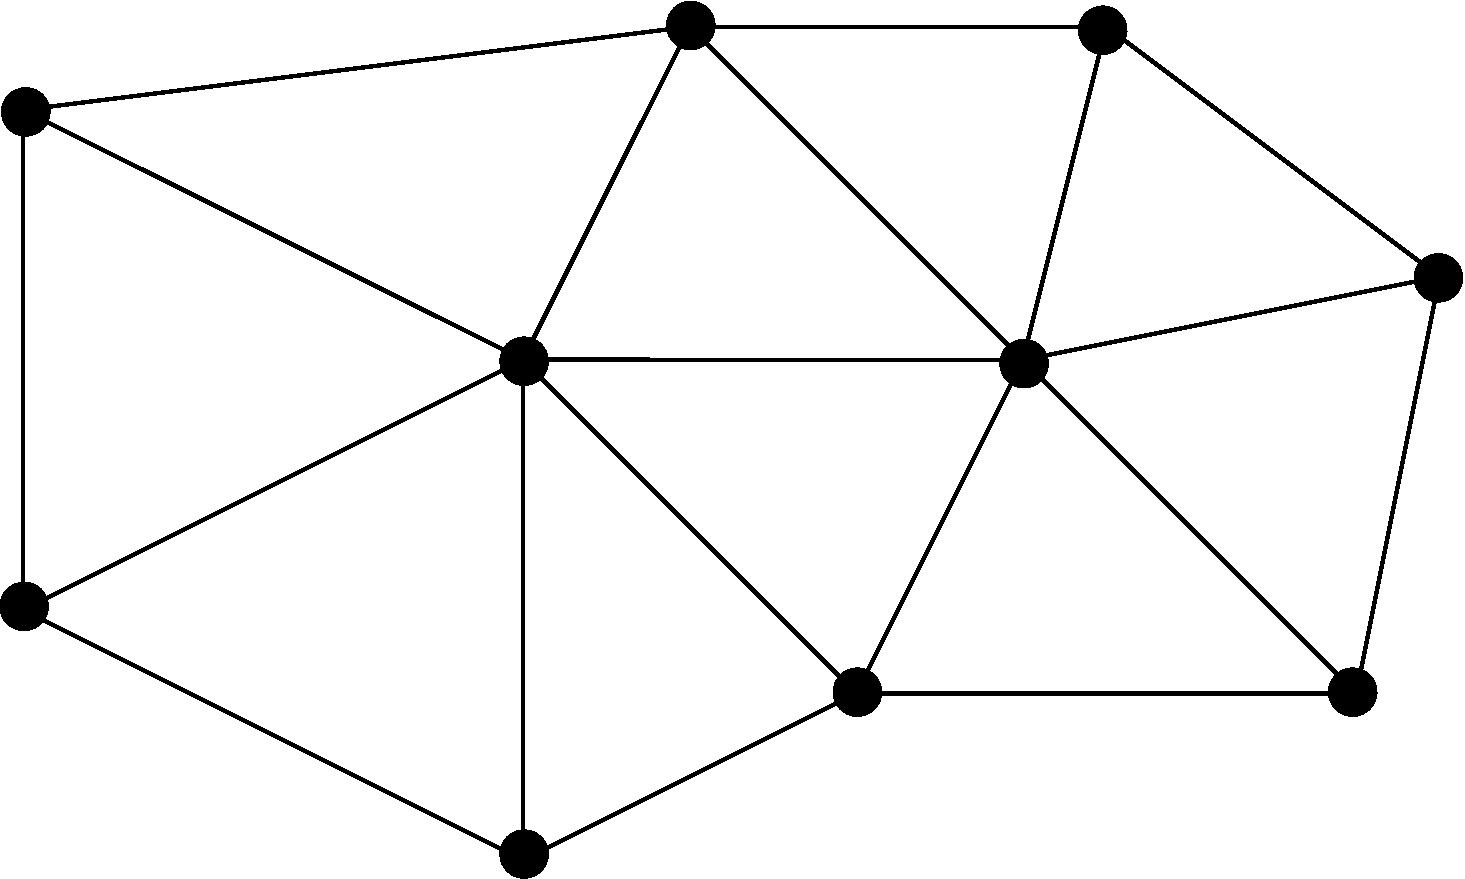
\includegraphics[width=\textwidth]{pdf/mesh-p1.pdf}
  \end{center}

\end{frame}

\begin{frame}
  \frametitle{The linear Lagrange element: $V_h$}

  \begin{center}
    \def\svgwidth{0.8\textwidth}
    \import{pdf/}{pdf/tri.pdf_tex}
  \end{center}

\end{frame}

\begin{frame}
  \frametitle{The quadratic Lagrange element: $(T, \mathcal{V}, \mathcal{L})$}

  \begin{itemize}
  \item
    $T$ is a line, triangle or tetrahedron
  \item
    $\mathcal{V}$ is the second-degree polynomials on $T$
  \item
    $\mathcal{L}$ is point evaluation at the vertices and edge midpoints
  \end{itemize}

\end{frame}

\begin{frame}
  \frametitle{The quadratic Lagrange element: $\mathcal{L}$}

  \begin{center}
    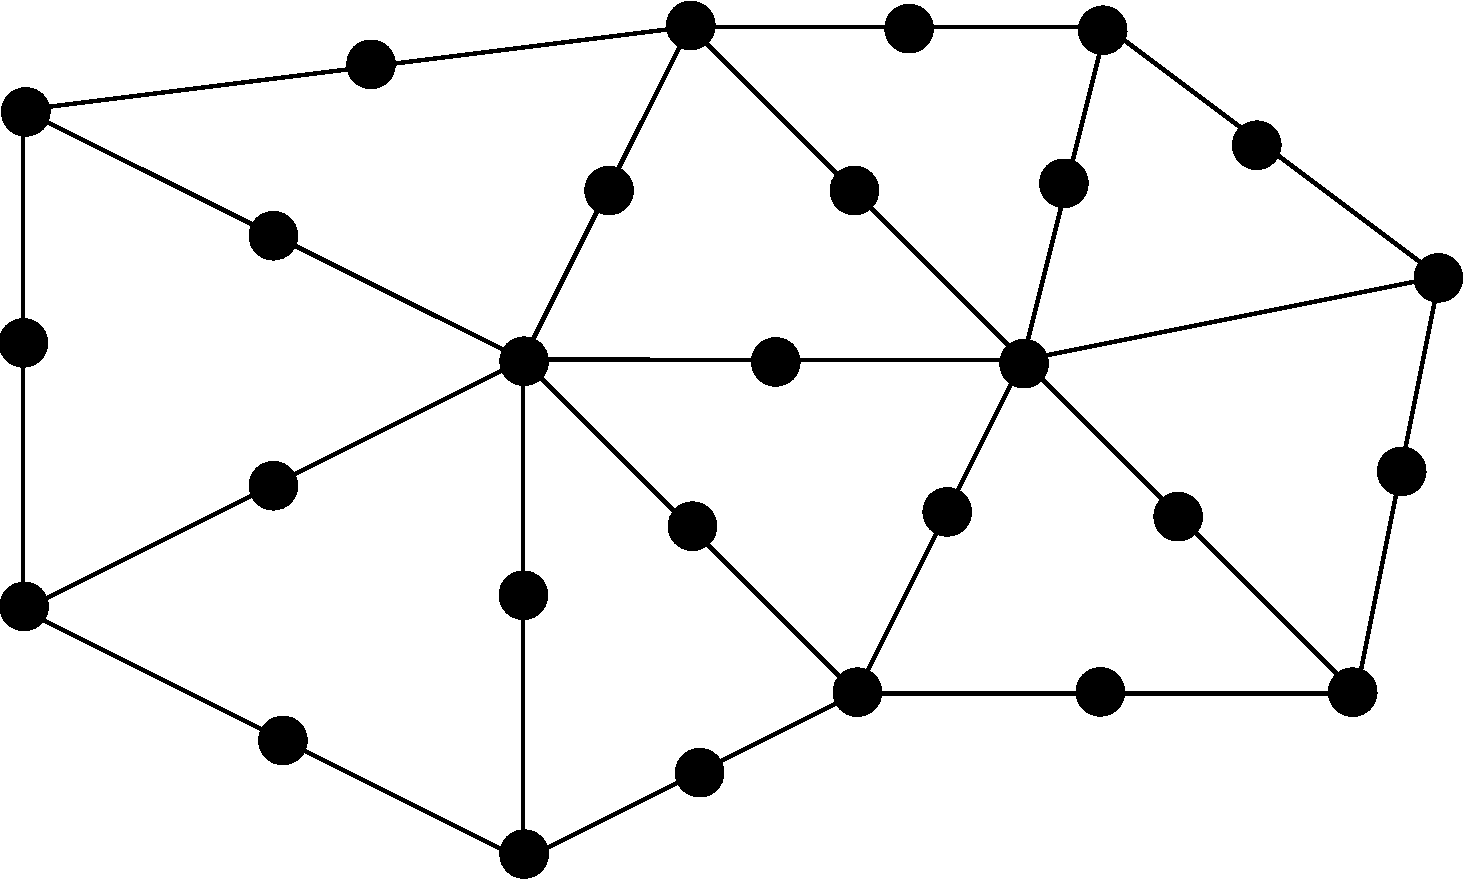
\includegraphics[width=\textwidth]{pdf/mesh-p2.pdf}
  \end{center}

\end{frame}

\begin{frame}
  \frametitle{The quadratic Lagrange element: $V_h$}

  \begin{center}
    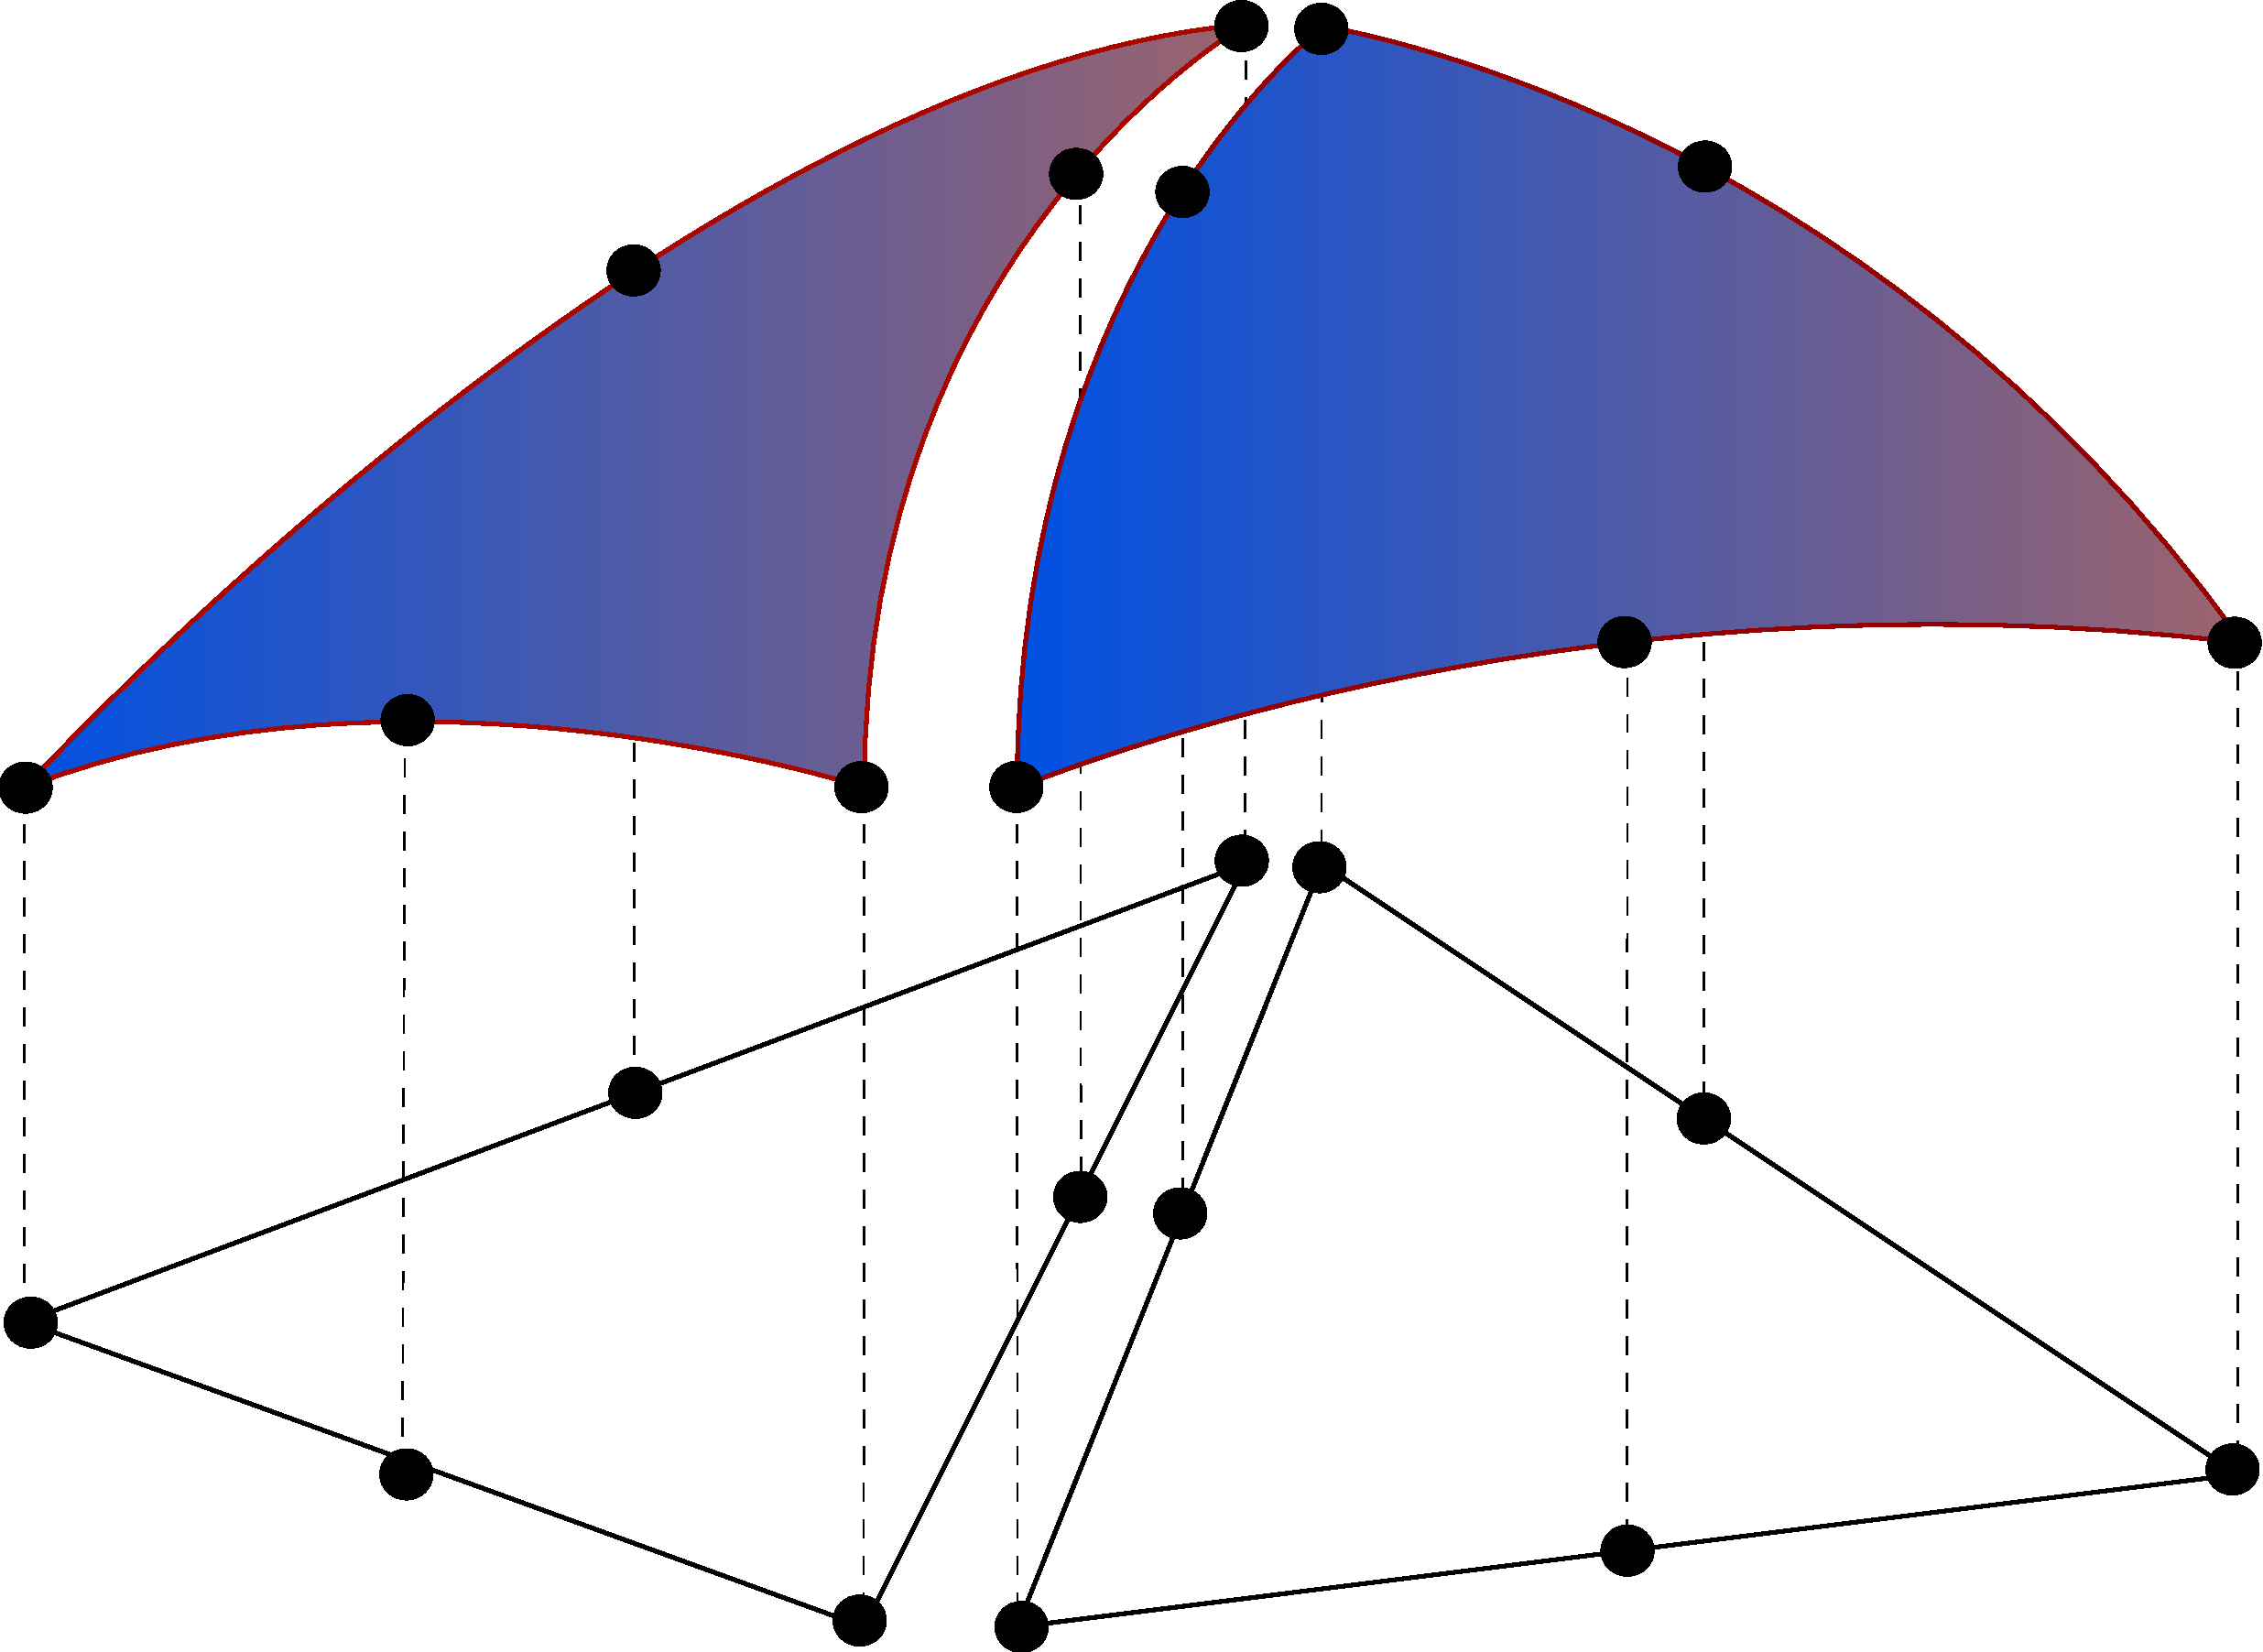
\includegraphics[width=0.9\textwidth]{pdf/femspace.pdf}
  \end{center}

\end{frame}

\begin{frame}
  \frametitle{Families of elements}

  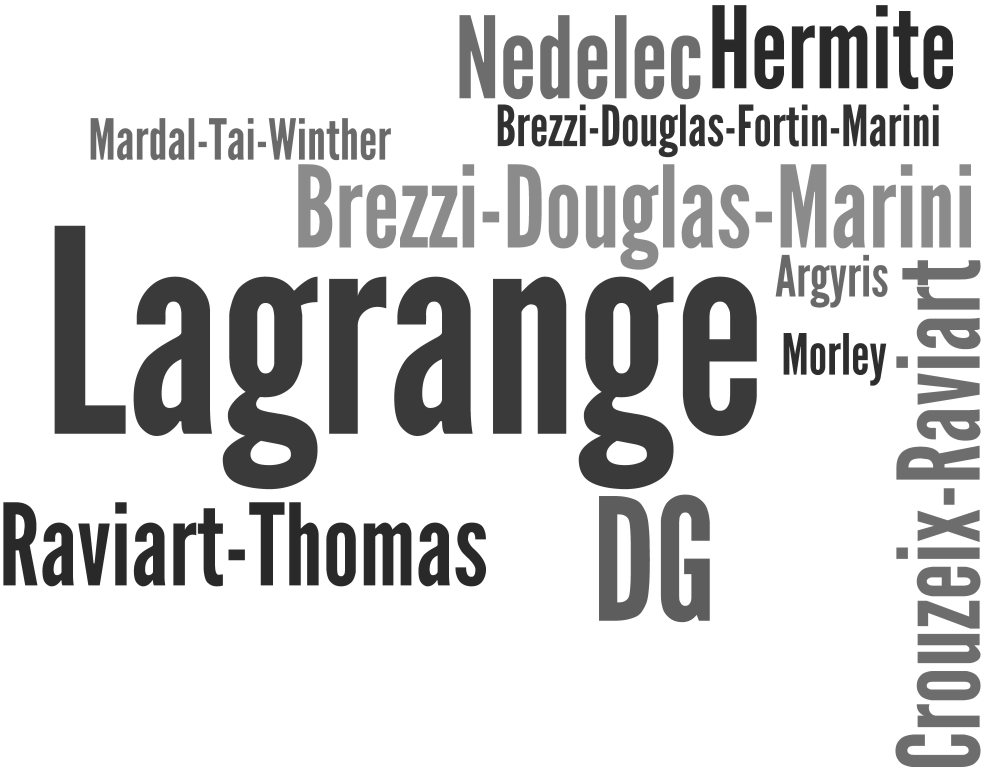
\includegraphics[width=0.9\textwidth]{png/elements_wordle.png}

\end{frame}

\begin{frame}
  \frametitle{Families of elements}

  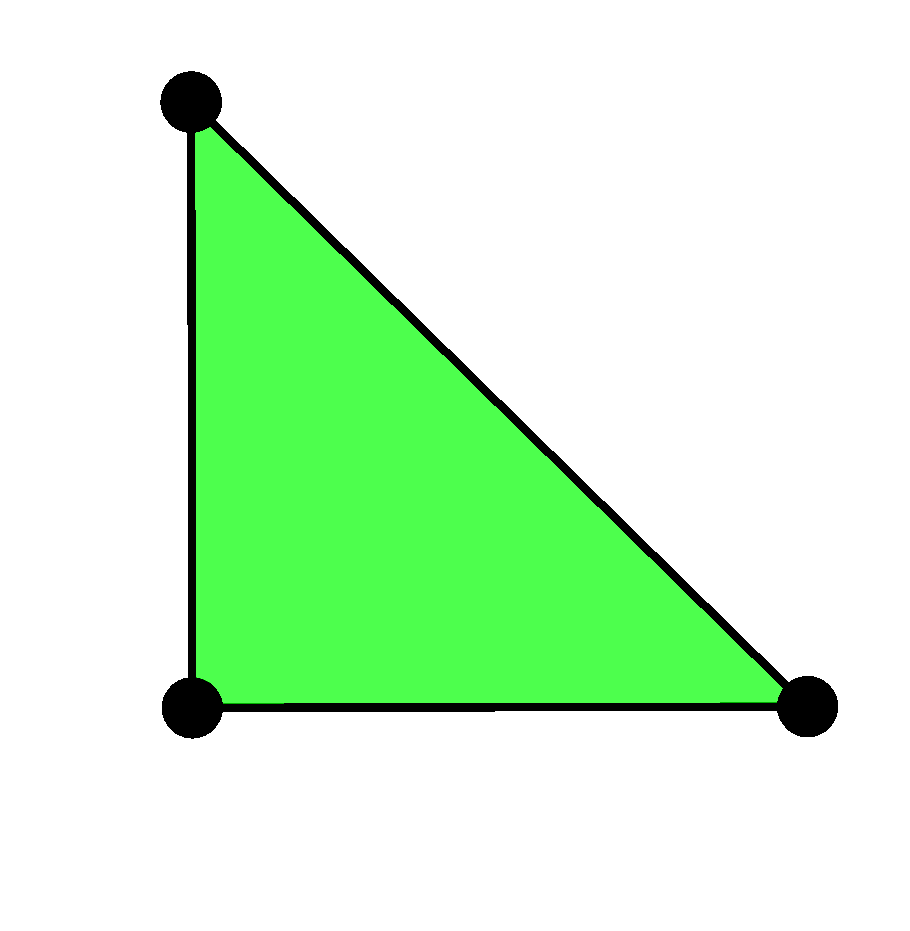
\includegraphics[width=1.3cm]{png/CG1_2d.png}
  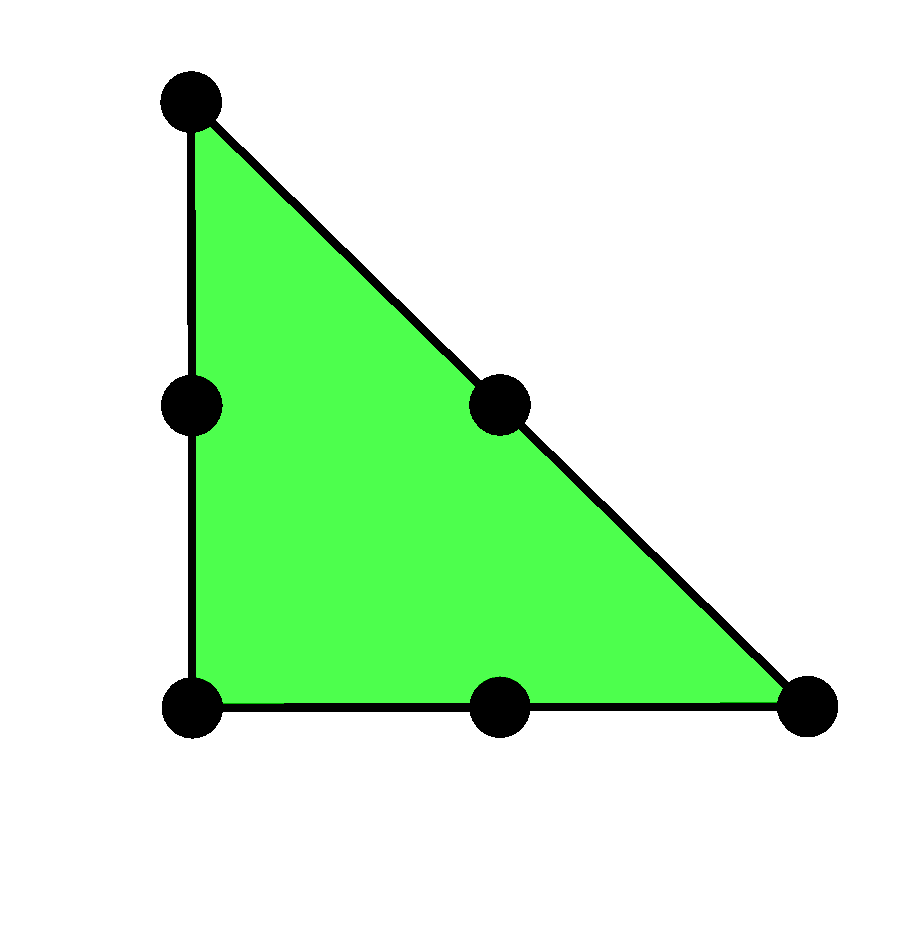
\includegraphics[width=1.3cm]{png/CG2_2d.png}
  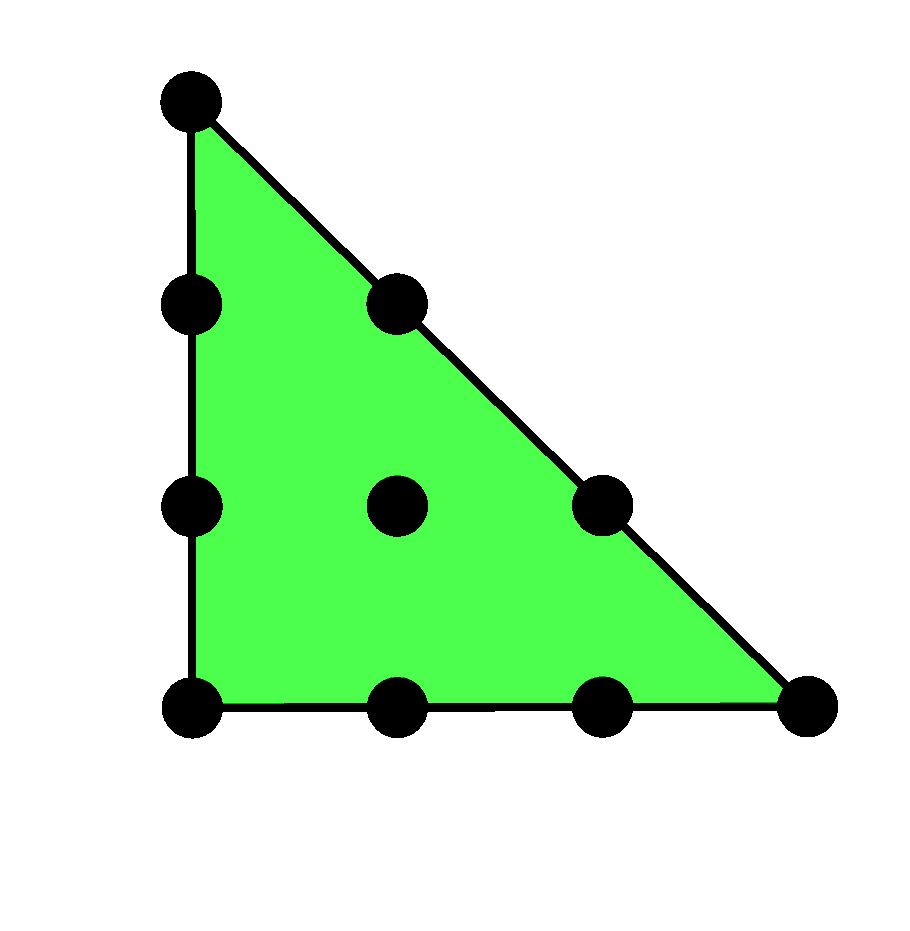
\includegraphics[width=1.3cm]{png/CG3_2d.png}
  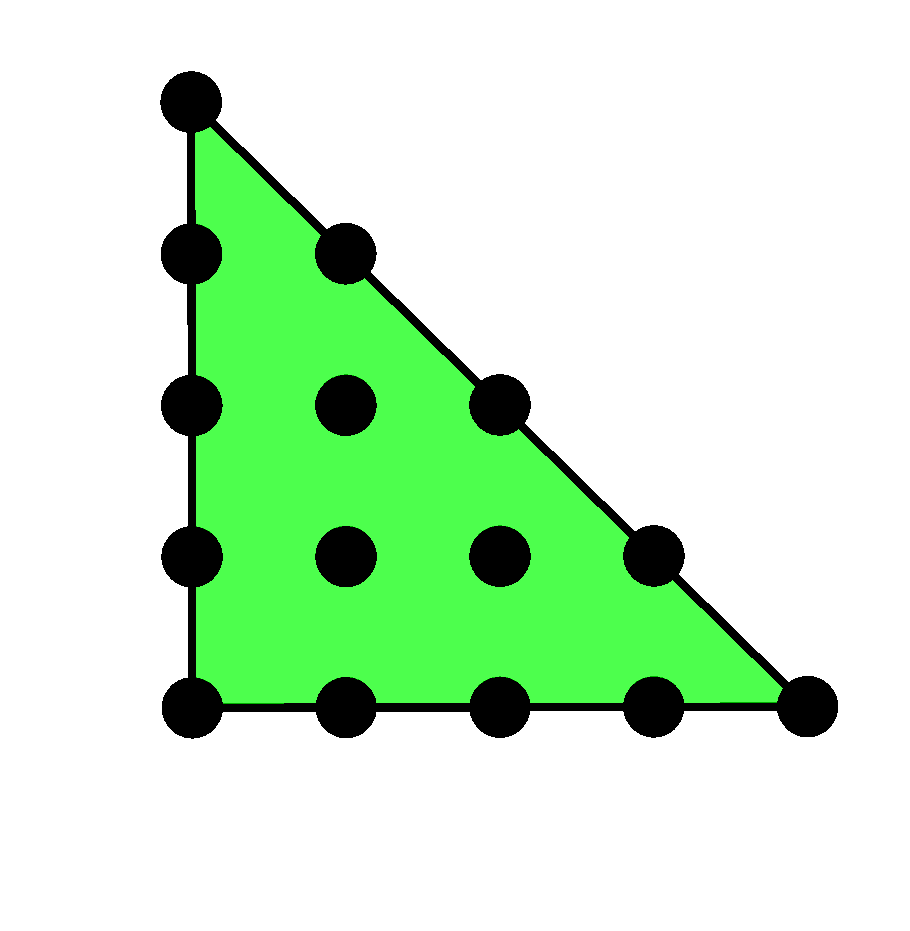
\includegraphics[width=1.3cm]{png/CG4_2d.png}
  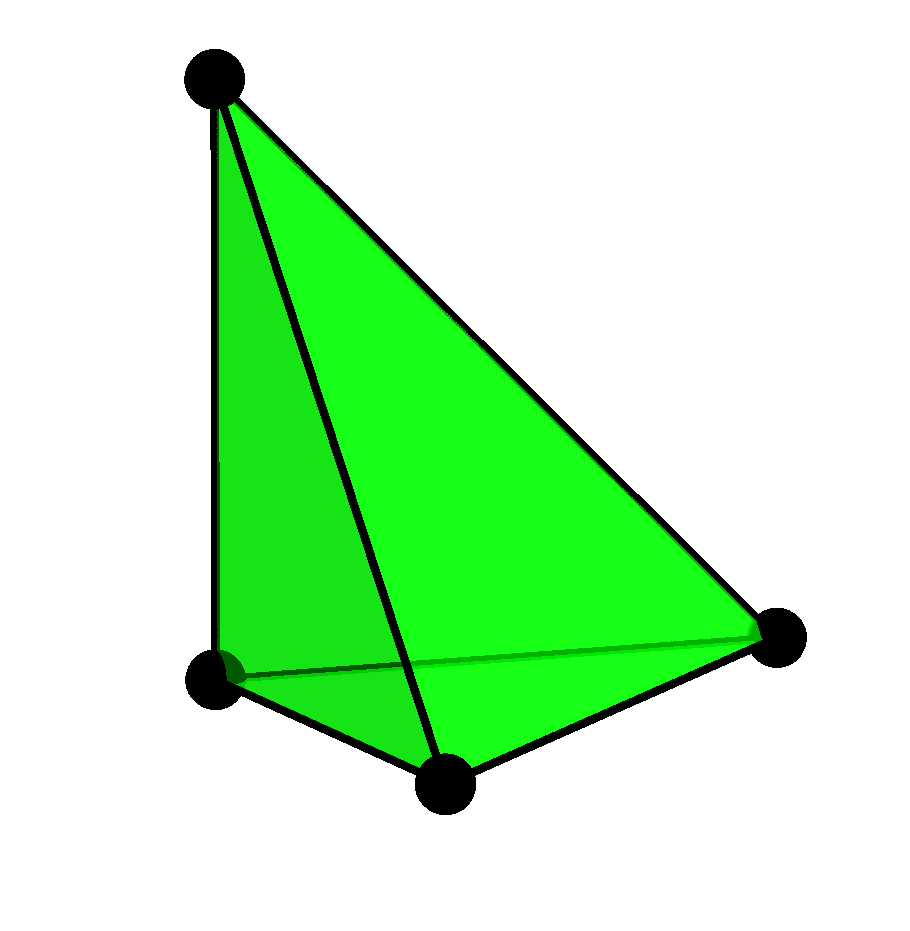
\includegraphics[width=1.3cm]{png/CG1_3d.png}
  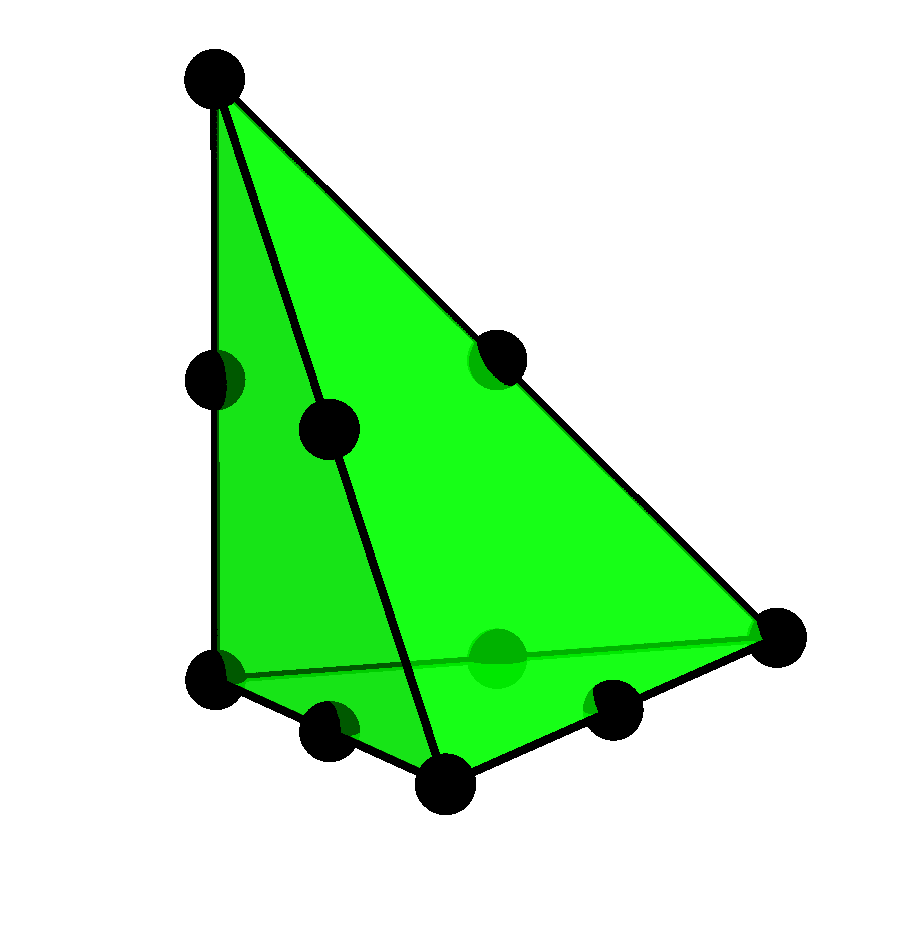
\includegraphics[width=1.3cm]{png/CG2_3d.png}
  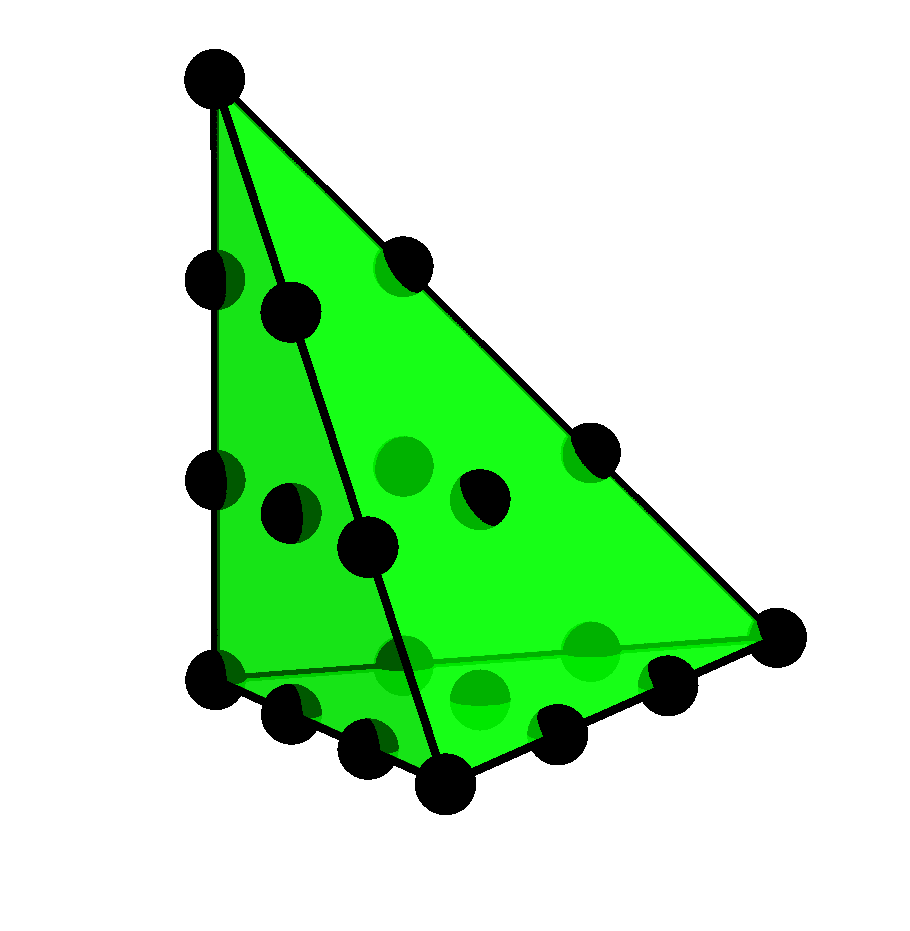
\includegraphics[width=1.3cm]{png/CG3_3d.png}
  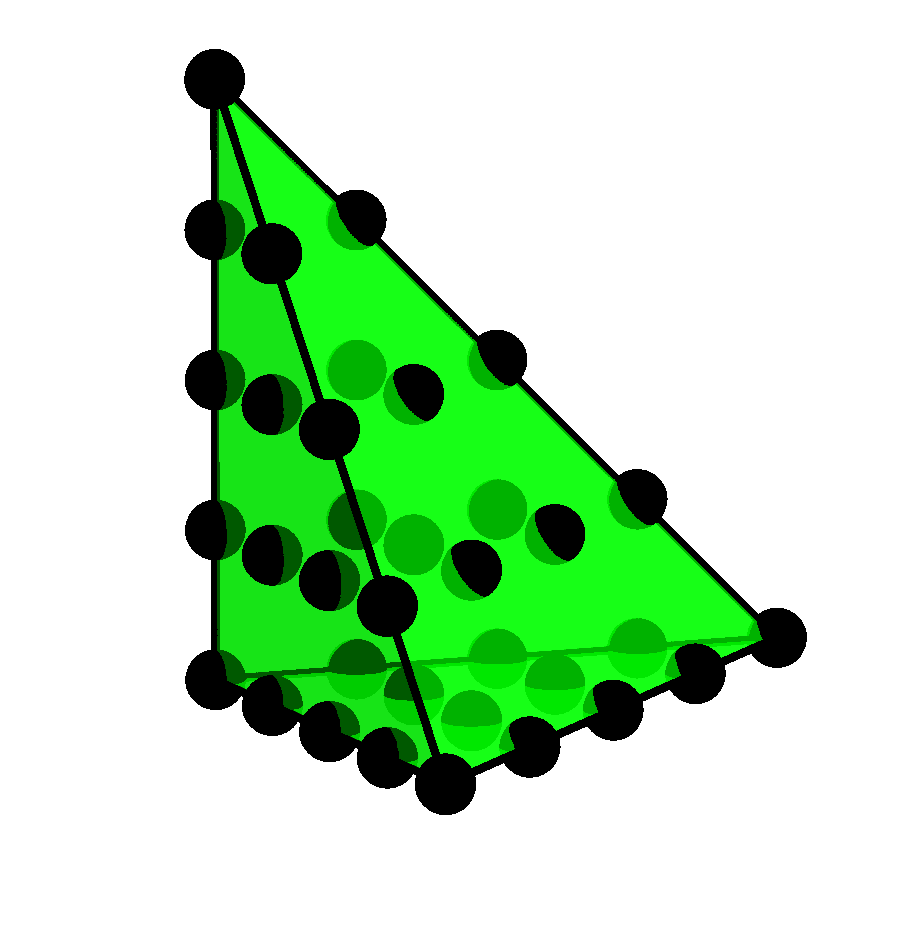
\includegraphics[width=1.3cm]{png/CG4_3d.png} \\
  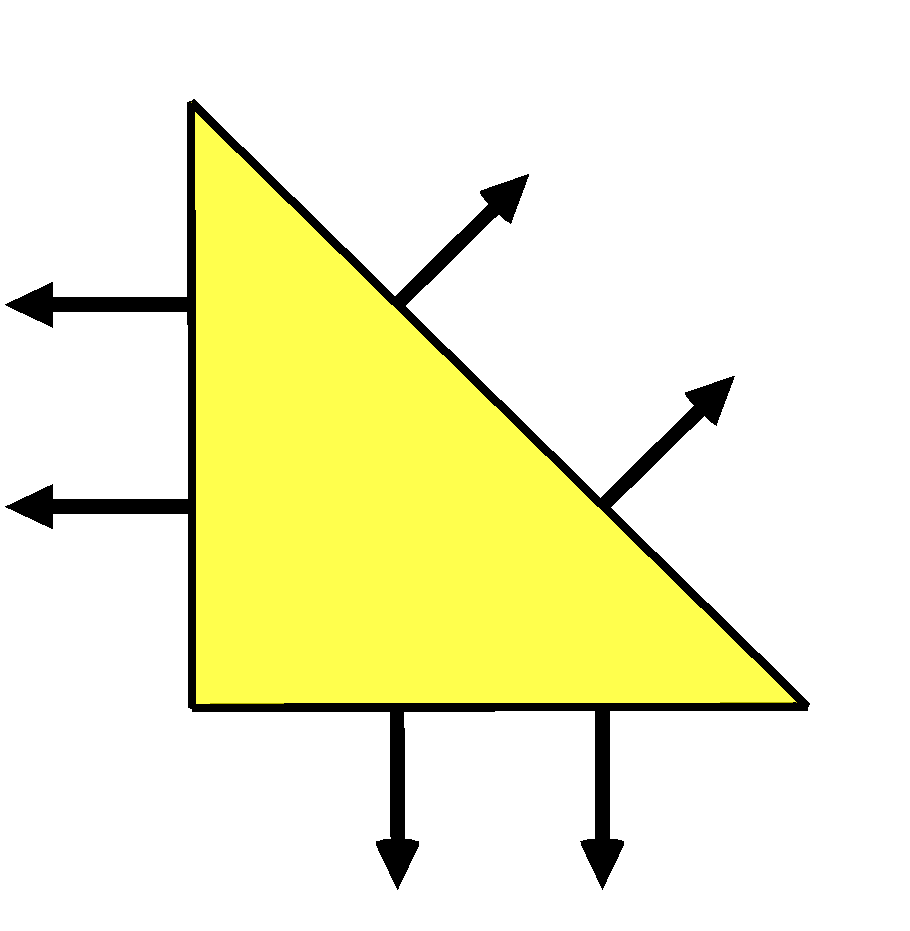
\includegraphics[width=1.3cm]{png/BDM1_2d.png}
  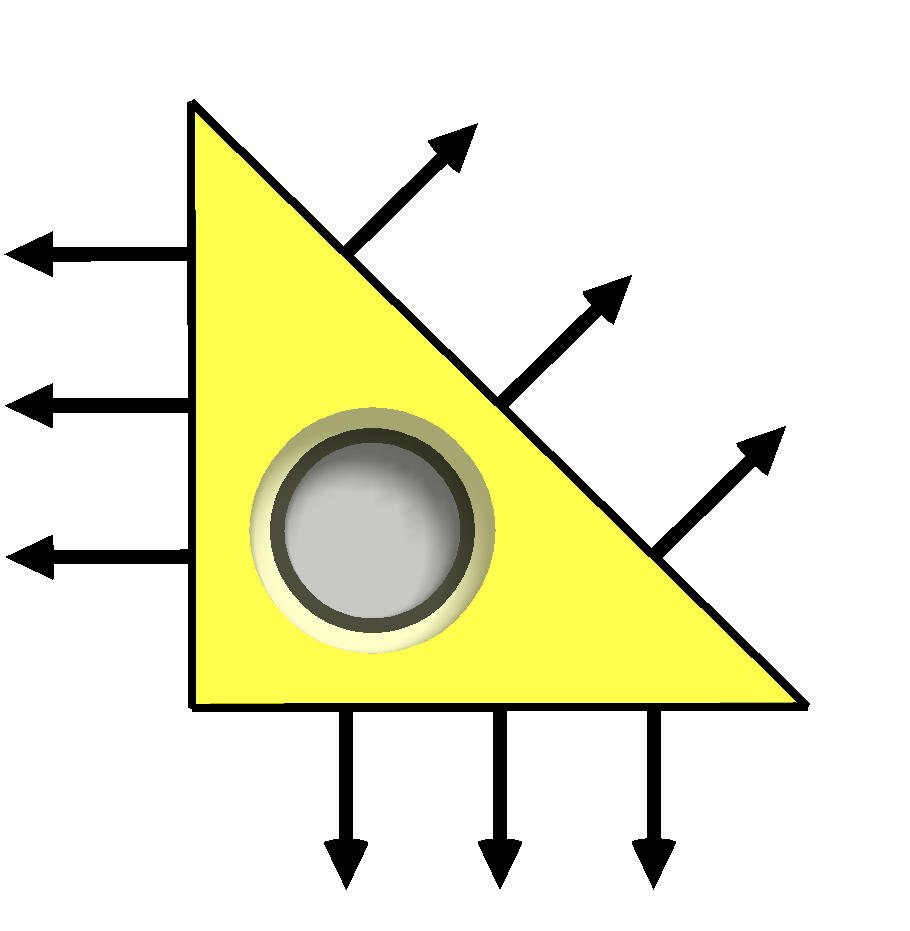
\includegraphics[width=1.3cm]{png/BDM2_2d.png}
  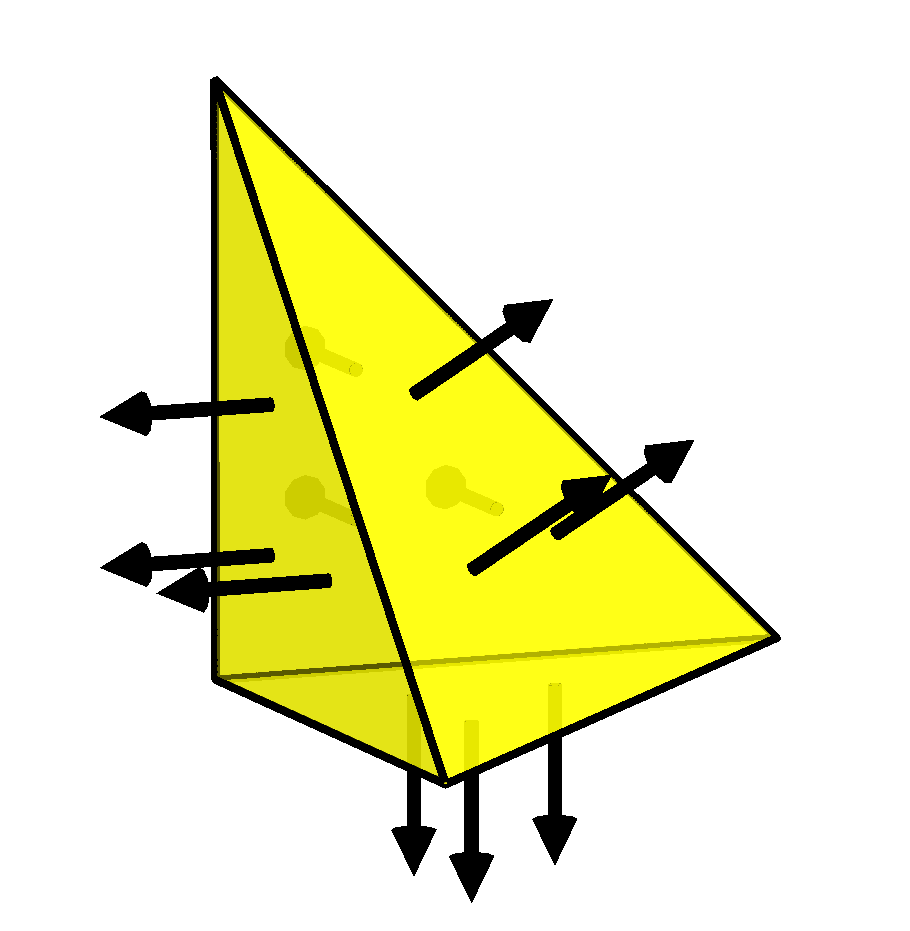
\includegraphics[width=1.3cm]{png/BDM1_3d.png}
  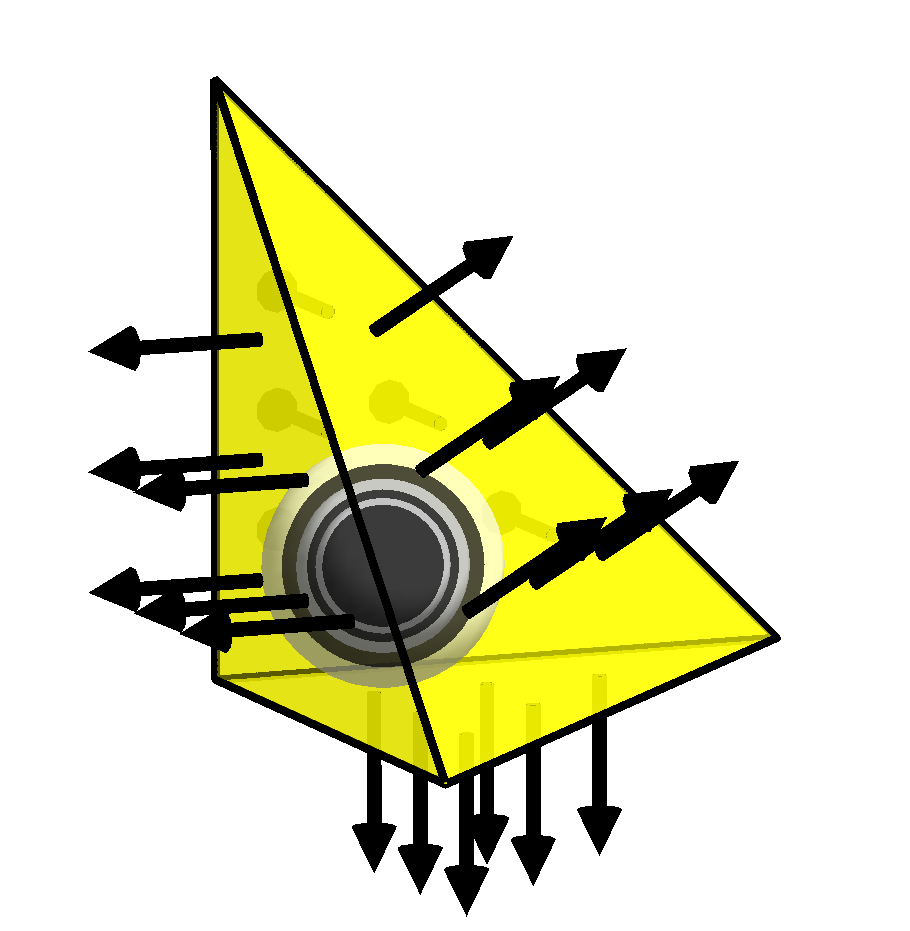
\includegraphics[width=1.3cm]{png/BDM2_3d.png}
  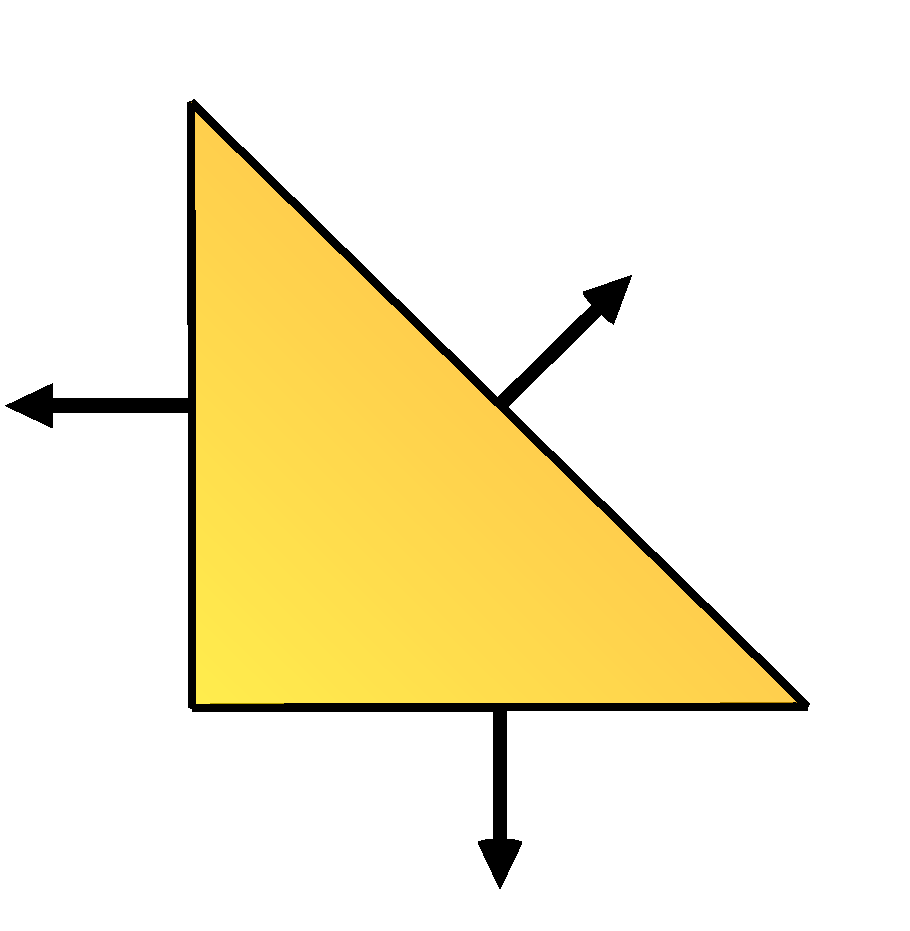
\includegraphics[width=1.3cm]{png/RT1_2d.png}
  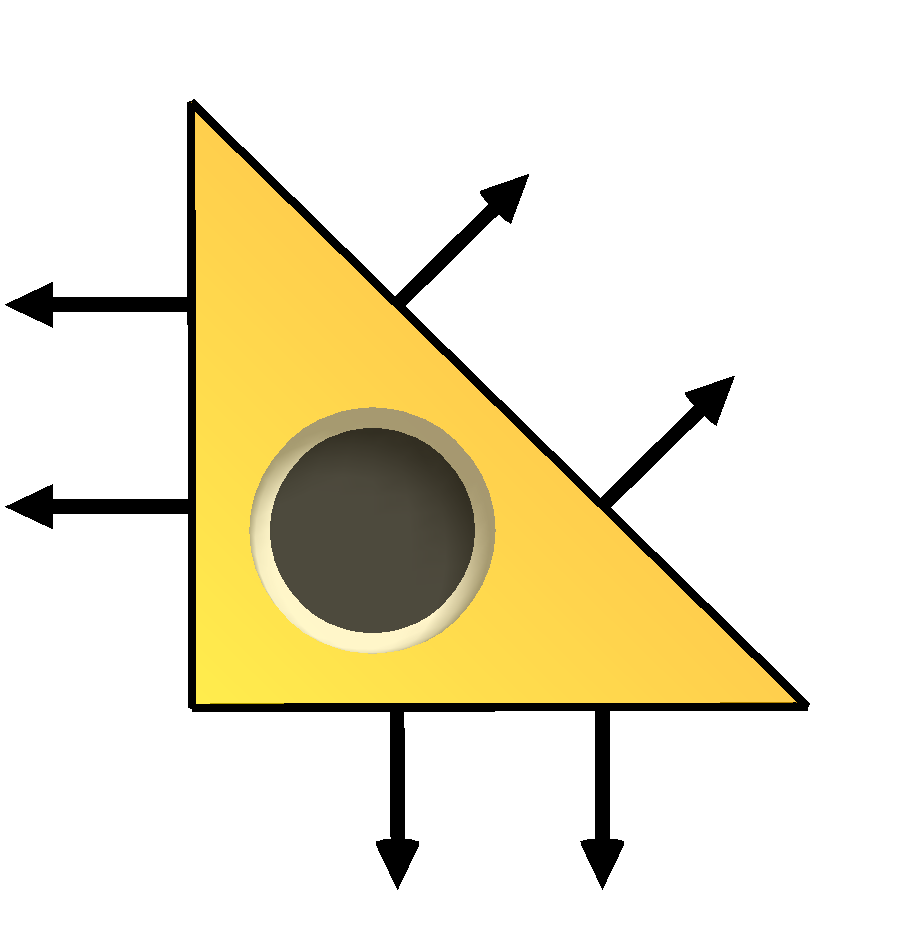
\includegraphics[width=1.3cm]{png/RT2_2d.png}
  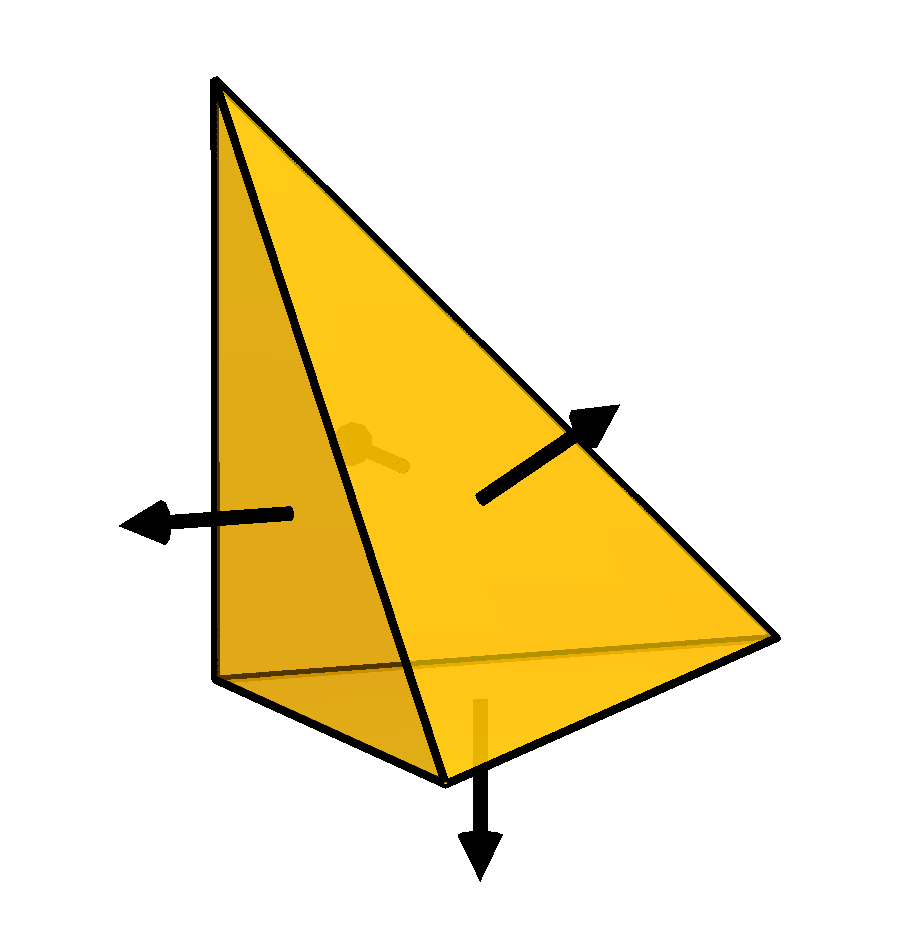
\includegraphics[width=1.3cm]{png/RT1_3d.png}
  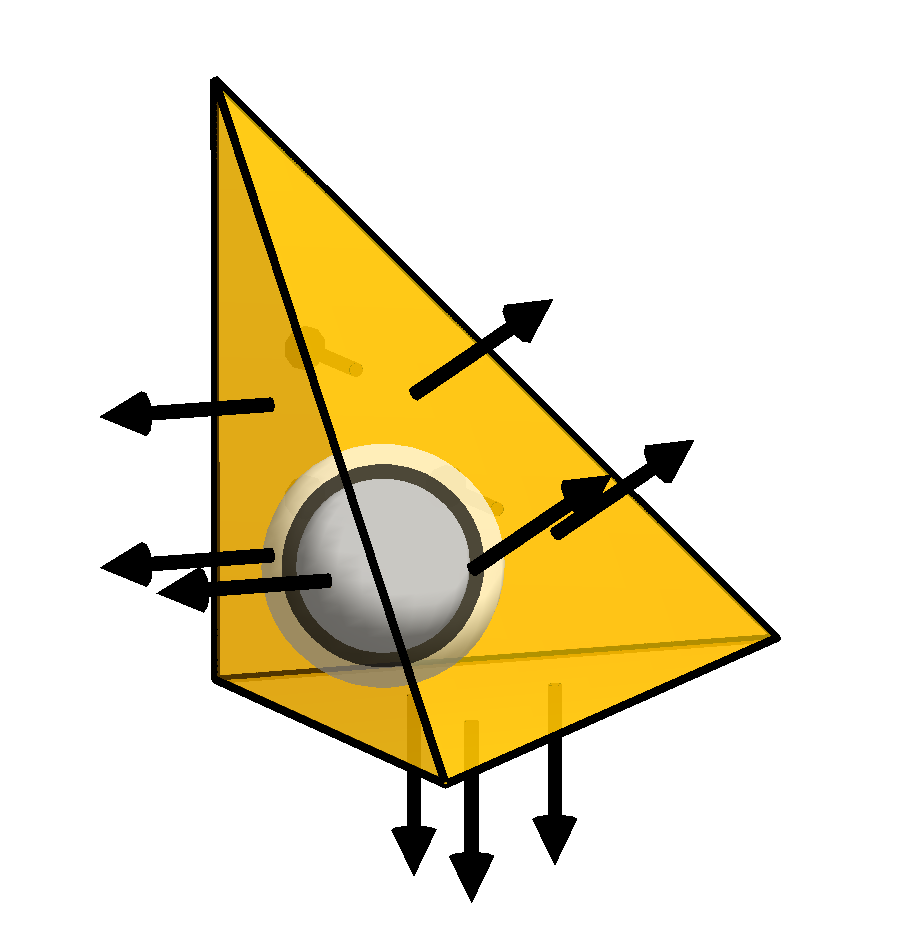
\includegraphics[width=1.3cm]{png/RT2_3d.png} \\
  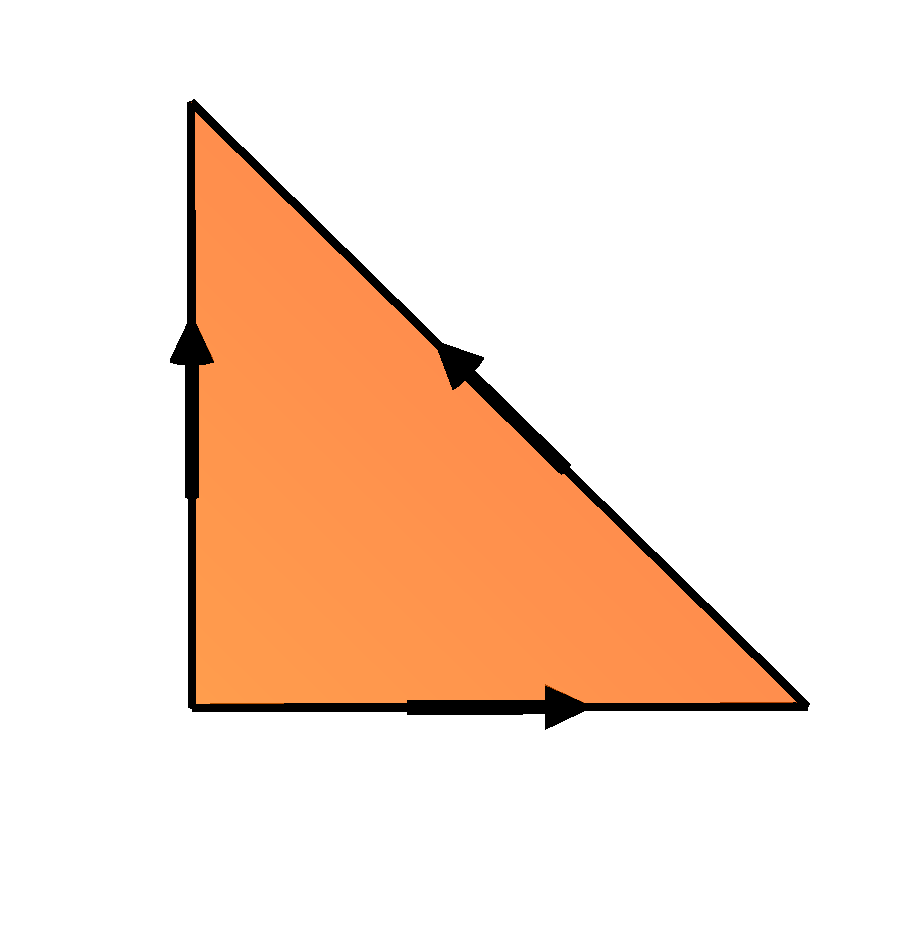
\includegraphics[width=1.3cm]{png/NED1_1_2d.png}
  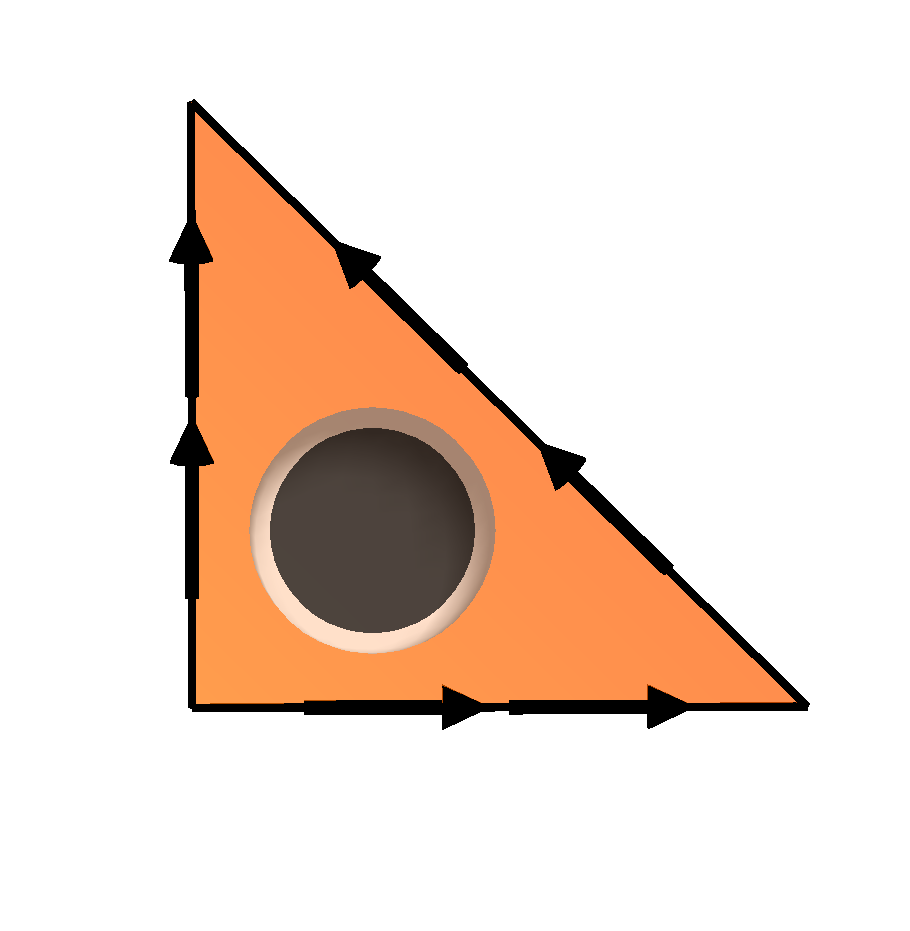
\includegraphics[width=1.3cm]{png/NED1_2_2d.png}
  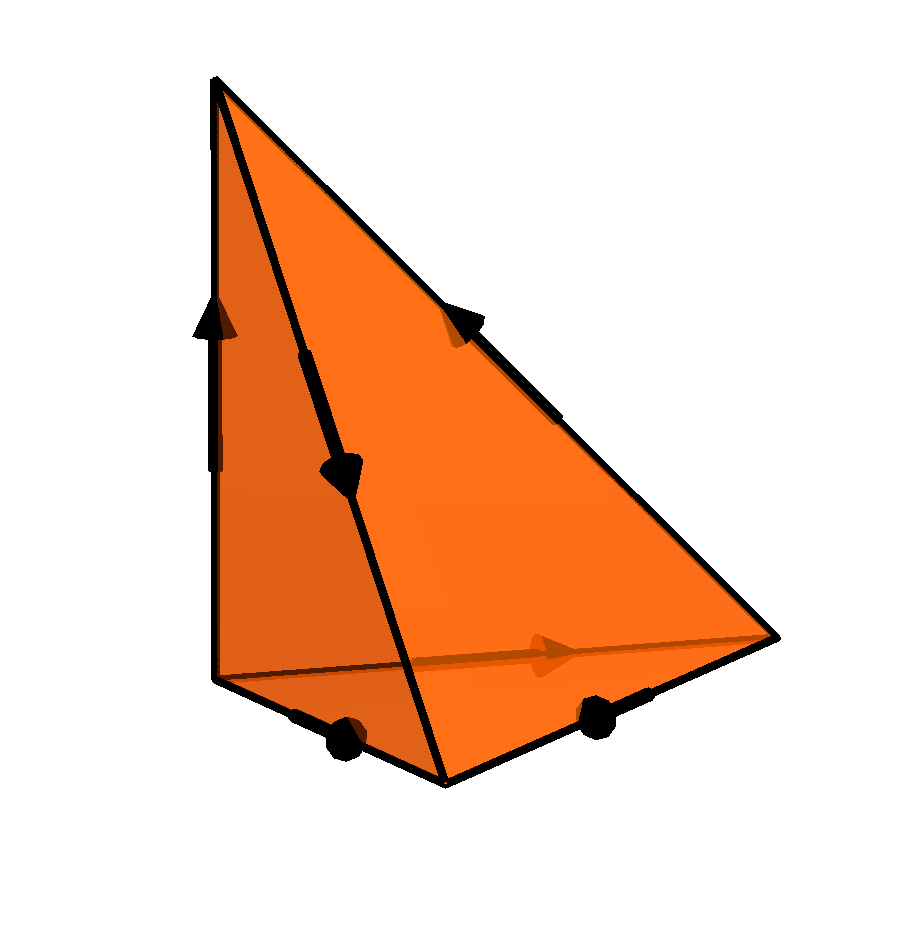
\includegraphics[width=1.3cm]{png/NED1_1_3d.png}
  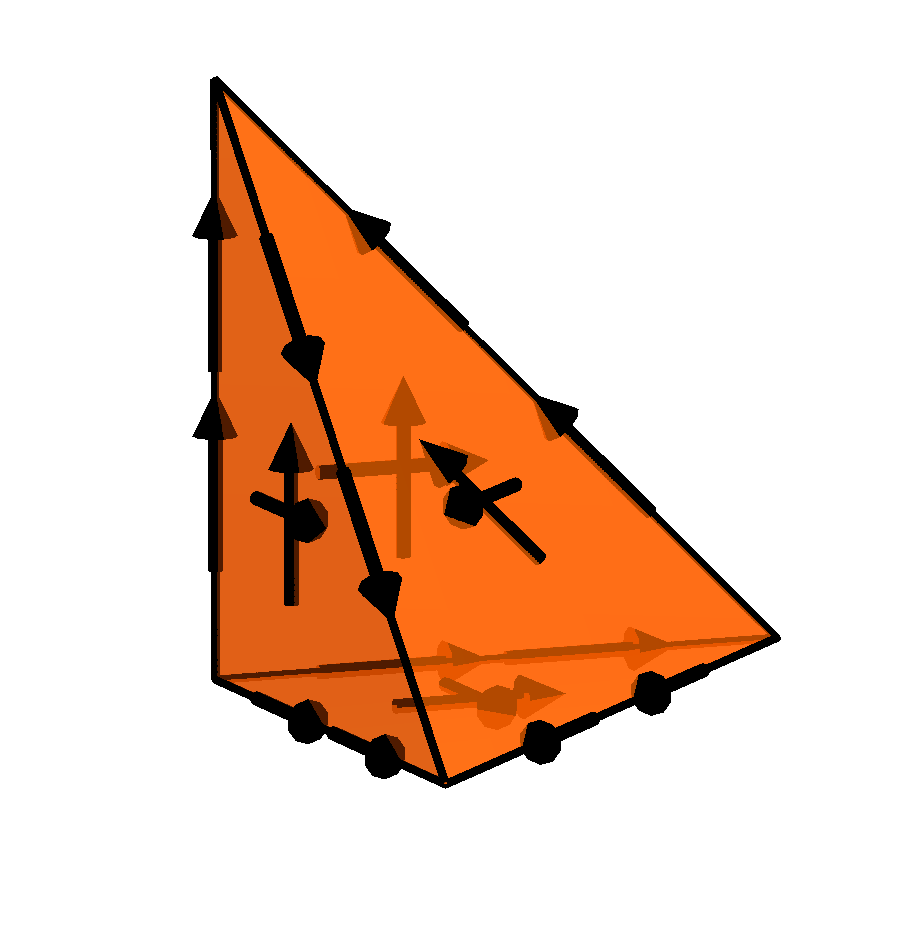
\includegraphics[width=1.3cm]{png/NED1_2_3d.png}
  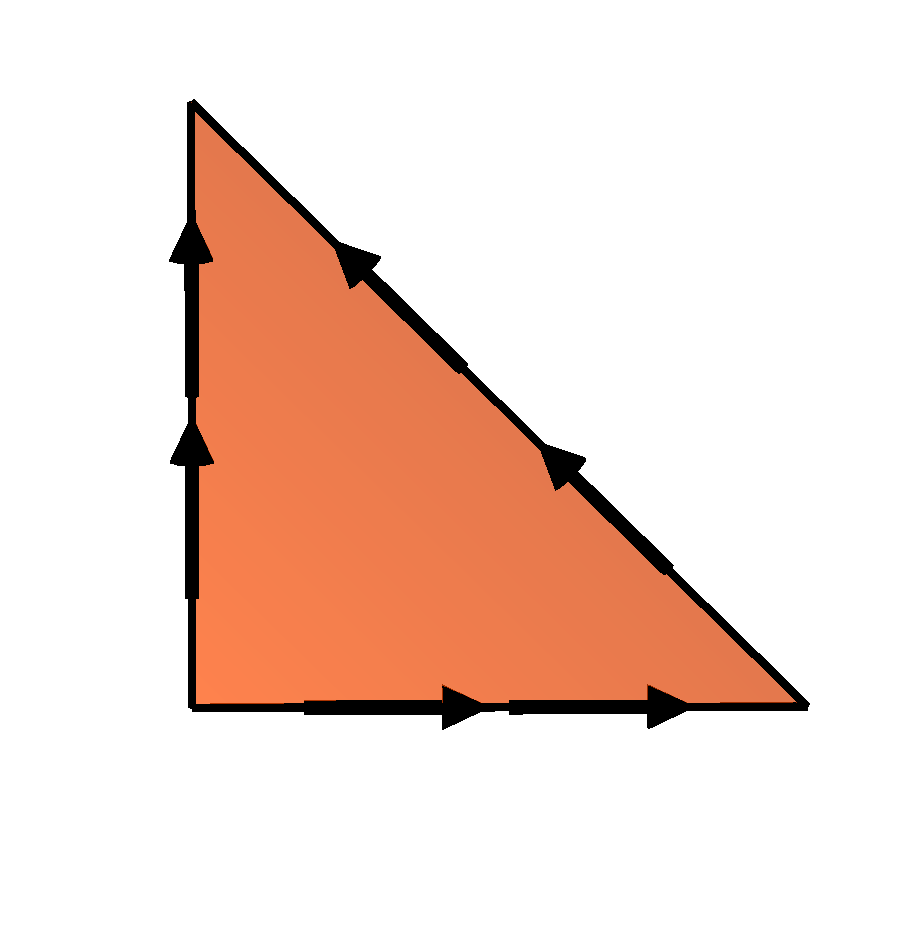
\includegraphics[width=1.3cm]{png/NED2_1_2d.png}
  
\includegraphics[width=1.3cm]{png/NED2_2_2d.png}
  
\includegraphics[width=1.3cm]{png/NED2_3_2d.png}
  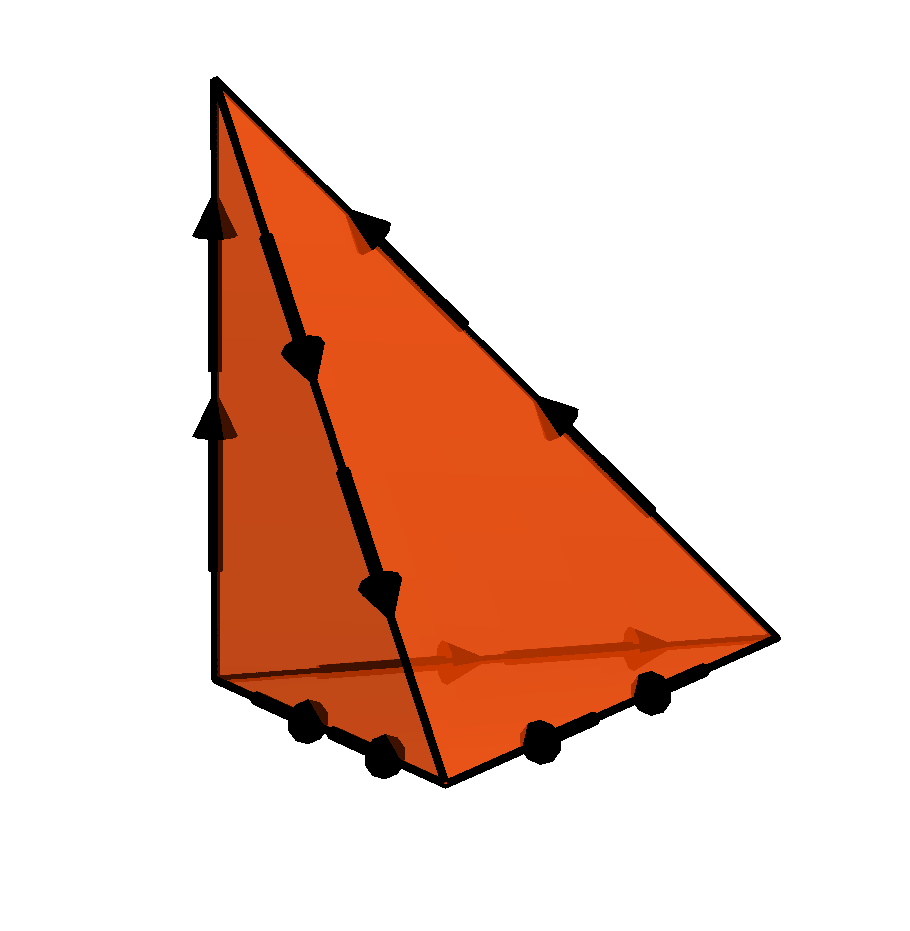
\includegraphics[width=1.3cm]{png/NED2_1_3d.png} \\
  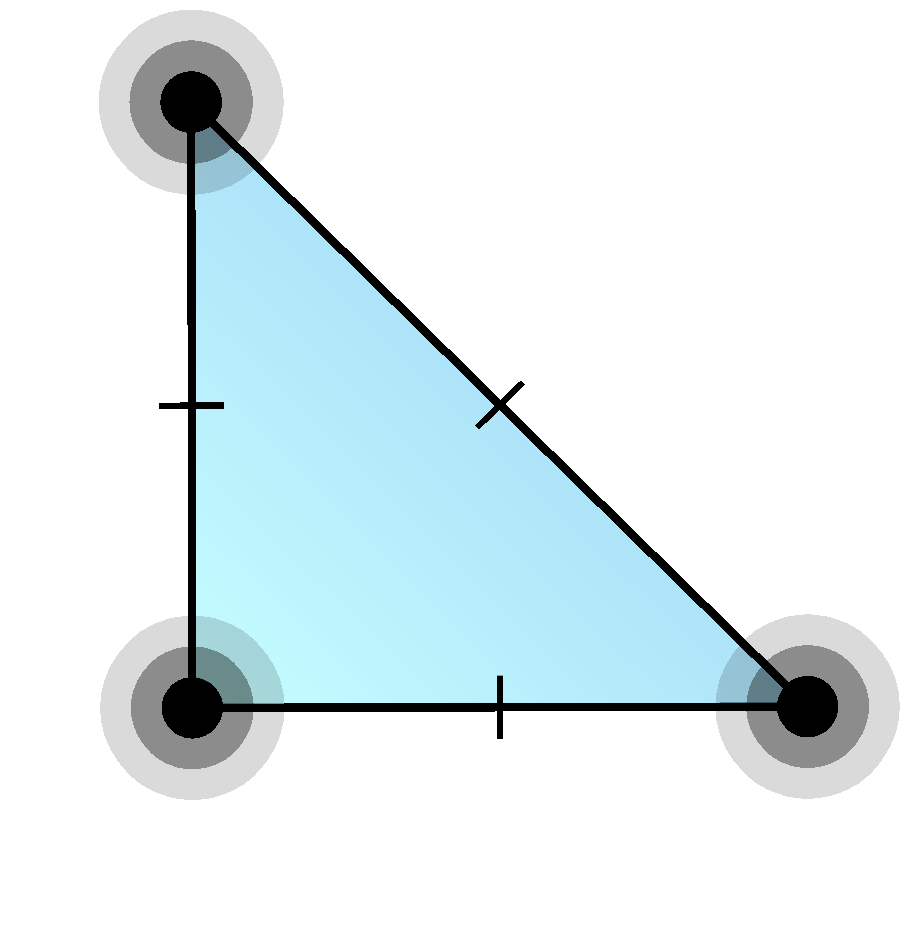
\includegraphics[width=1.3cm]{png/ARG5_2d.png}
  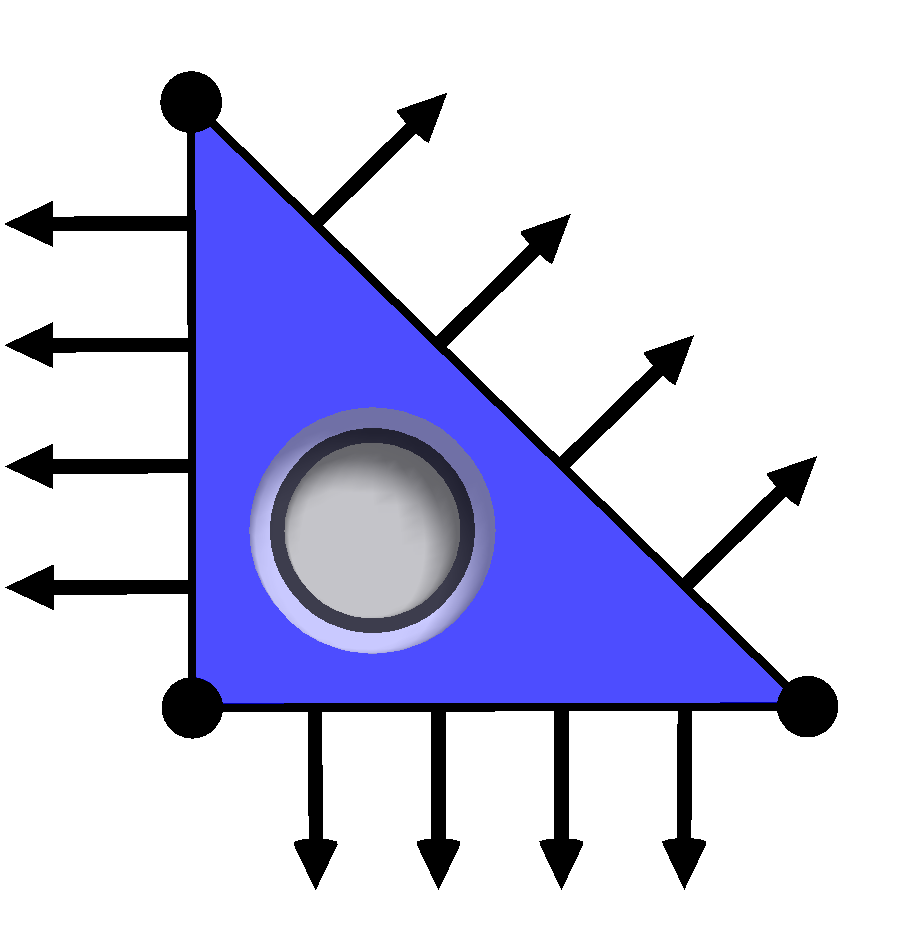
\includegraphics[width=1.3cm]{png/AW_2d.png}
  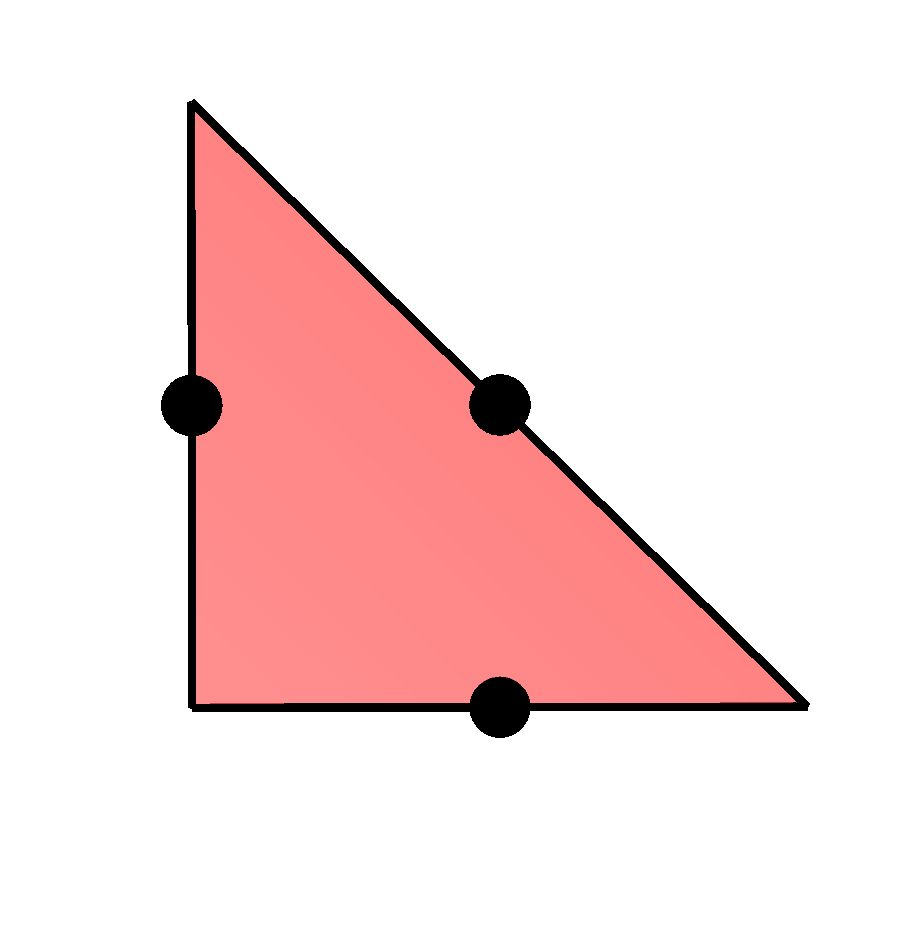
\includegraphics[width=1.3cm]{png/CR1_2d.png}
  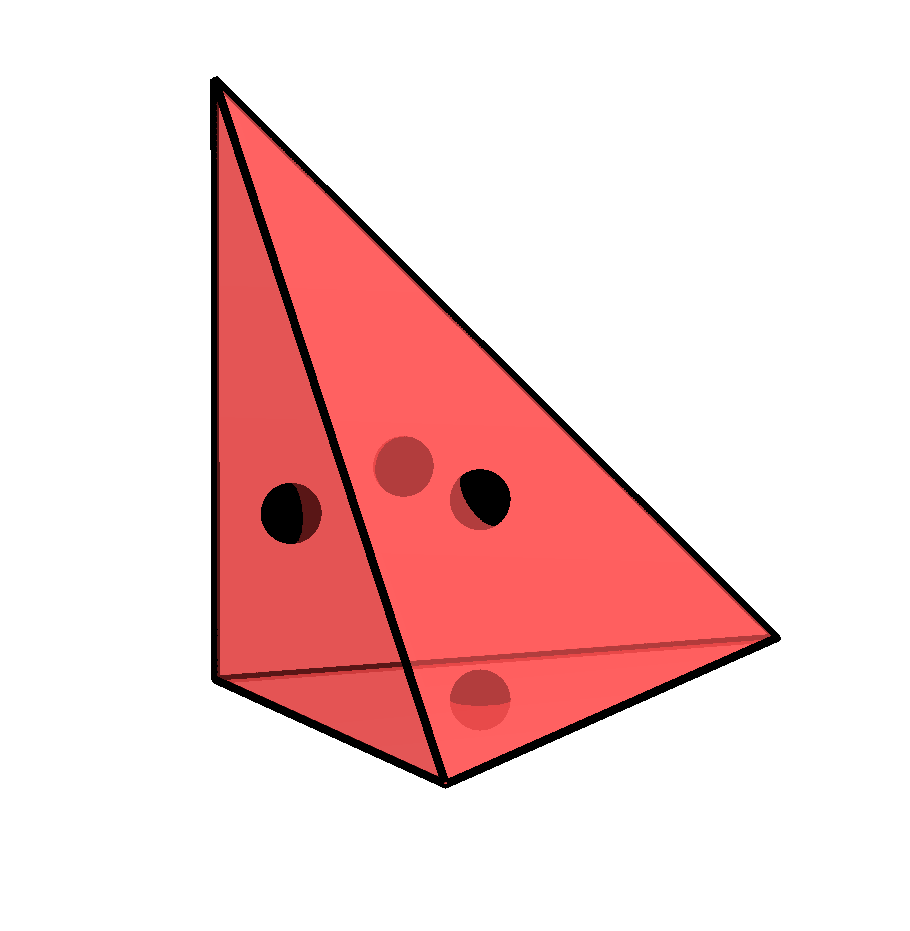
\includegraphics[width=1.3cm]{png/CR1_3d.png}
  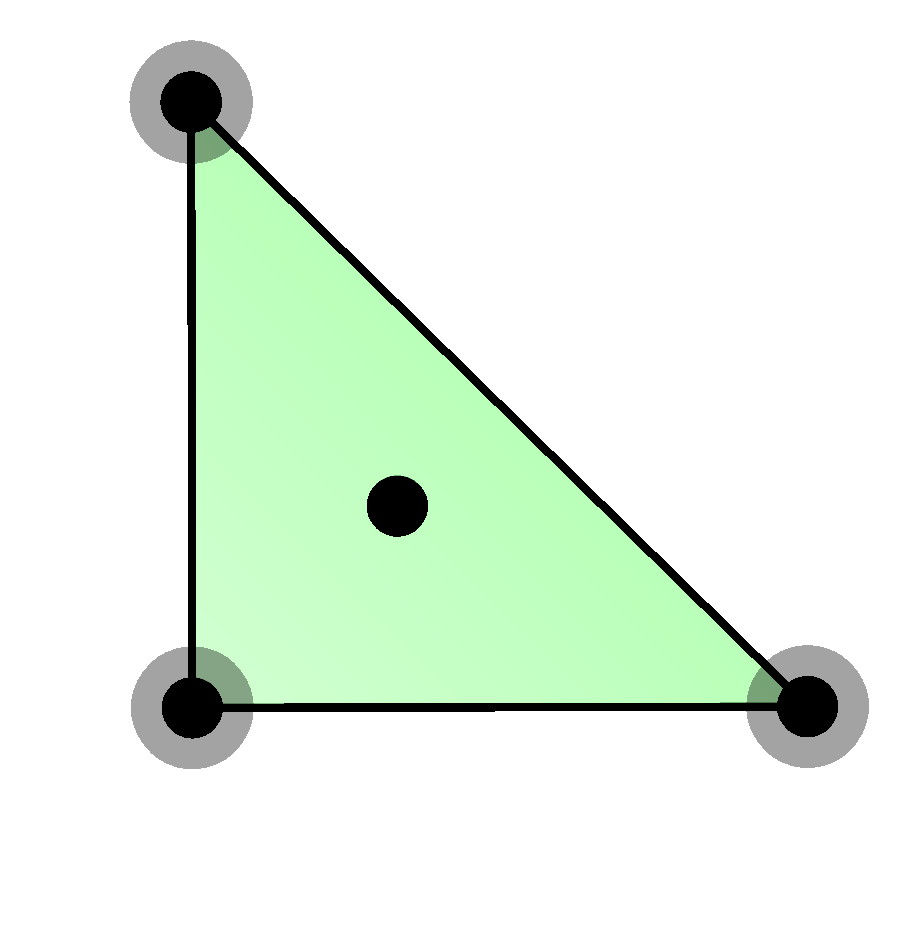
\includegraphics[width=1.3cm]{png/HER_2d.png}
  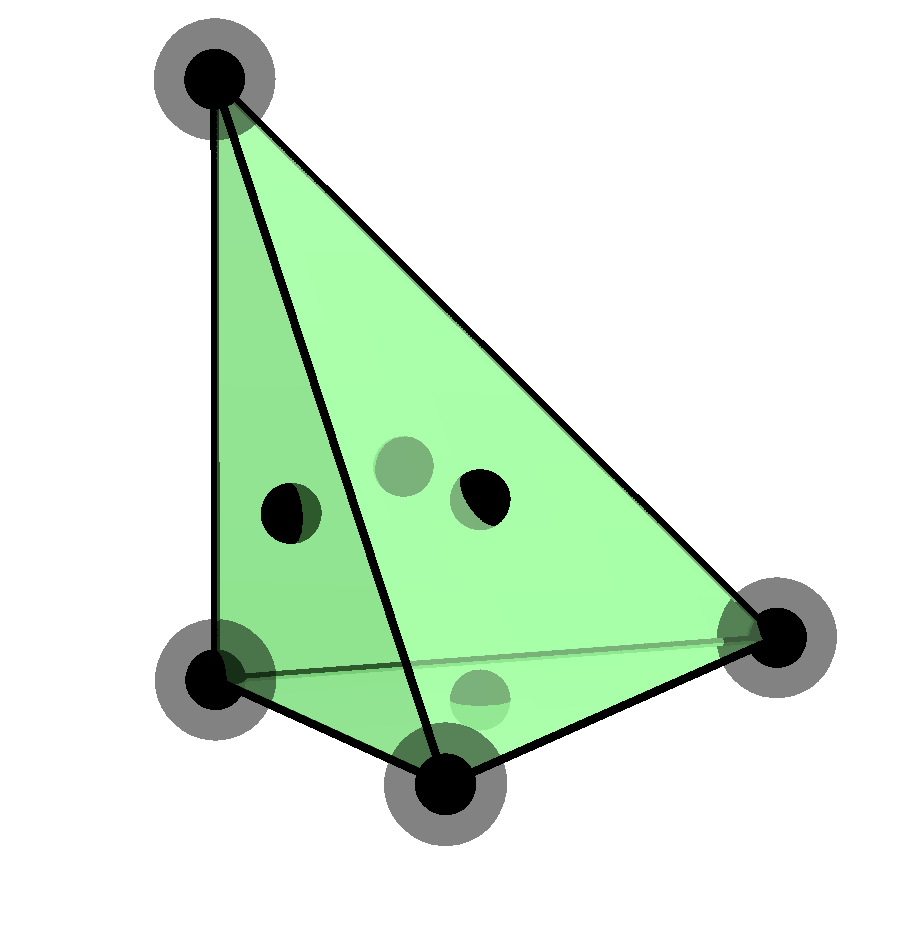
\includegraphics[width=1.3cm]{png/HER_3d.png}
  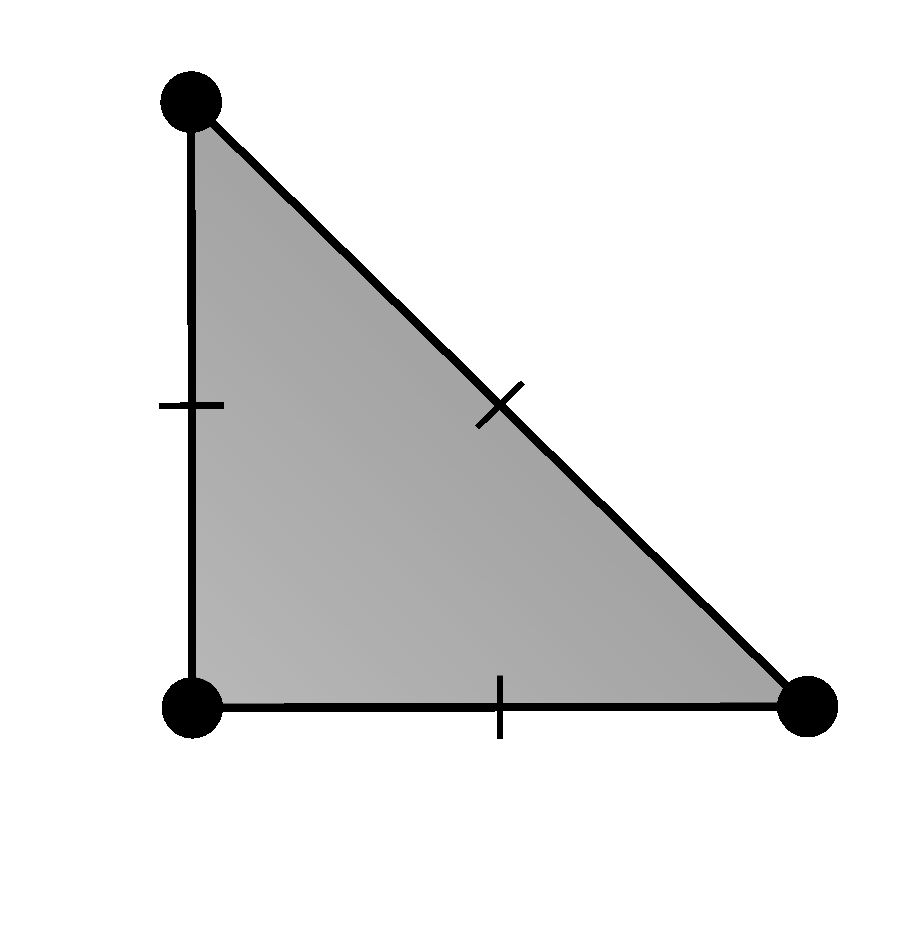
\includegraphics[width=1.3cm]{png/MOR_2d.png}
  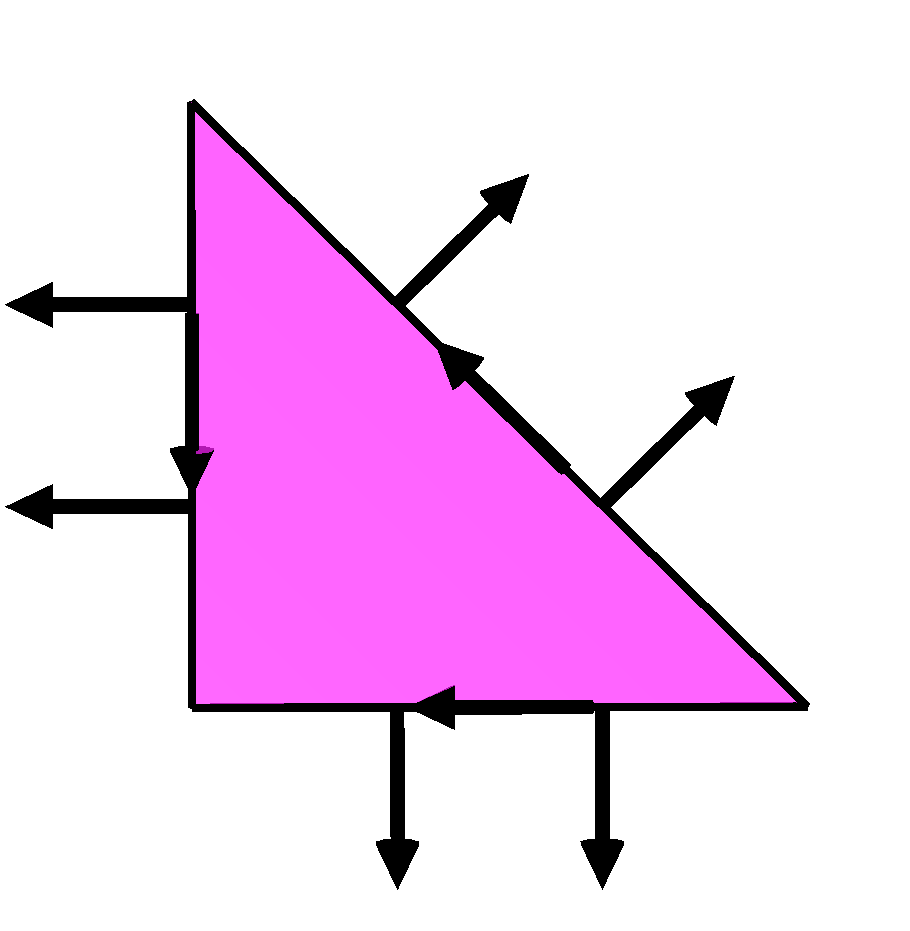
\includegraphics[width=1.3cm]{png/MTW_2d.png}

\end{frame}


\fenicssection{Computing the sparse matrix $A$}

\begin{frame}
  \frametitle{Why is the matrix sparse?}

\end{frame}

\begin{frame}
  \frametitle{Naive assembly algorithm}

  \begin{tabbing}
    $A = 0$ \\
    \\
    \textbf{for} $i=1,\ldots,N$ \\
    \\
    \tab \textbf{for} $j=1,\ldots,N$ \\
    \\
    \tab \tab $A_{ij} = a(\phi_j, \phi_i)$ \\
    \\
    \tab \textbf{end for} \\
    \\
    \textbf{end for}
  \end{tabbing}

\end{frame}

\begin{frame}
  \frametitle{The element matrix}

  The global matrix $A$ is defined by
  \begin{equation*}
    A_{ij} = a(\phi_j, \phi_i)
  \end{equation*}

  \bigskip

  The \emph{element matrix} $A_T$ is defined by
  \begin{equation*}
    A_{T,ij} = a_T(\phi_j^T, \phi_i^T)
  \end{equation*}

\end{frame}

\begin{frame}
  \frametitle{The local-to-global mapping}

  The global matrix $\iota_T$ is defined by
  \begin{equation*}
    I = \iota_T(i)
  \end{equation*}
  where $I$ is the \emph{global index} corresponding to
  the \emph{local index} i

  \begin{center}
    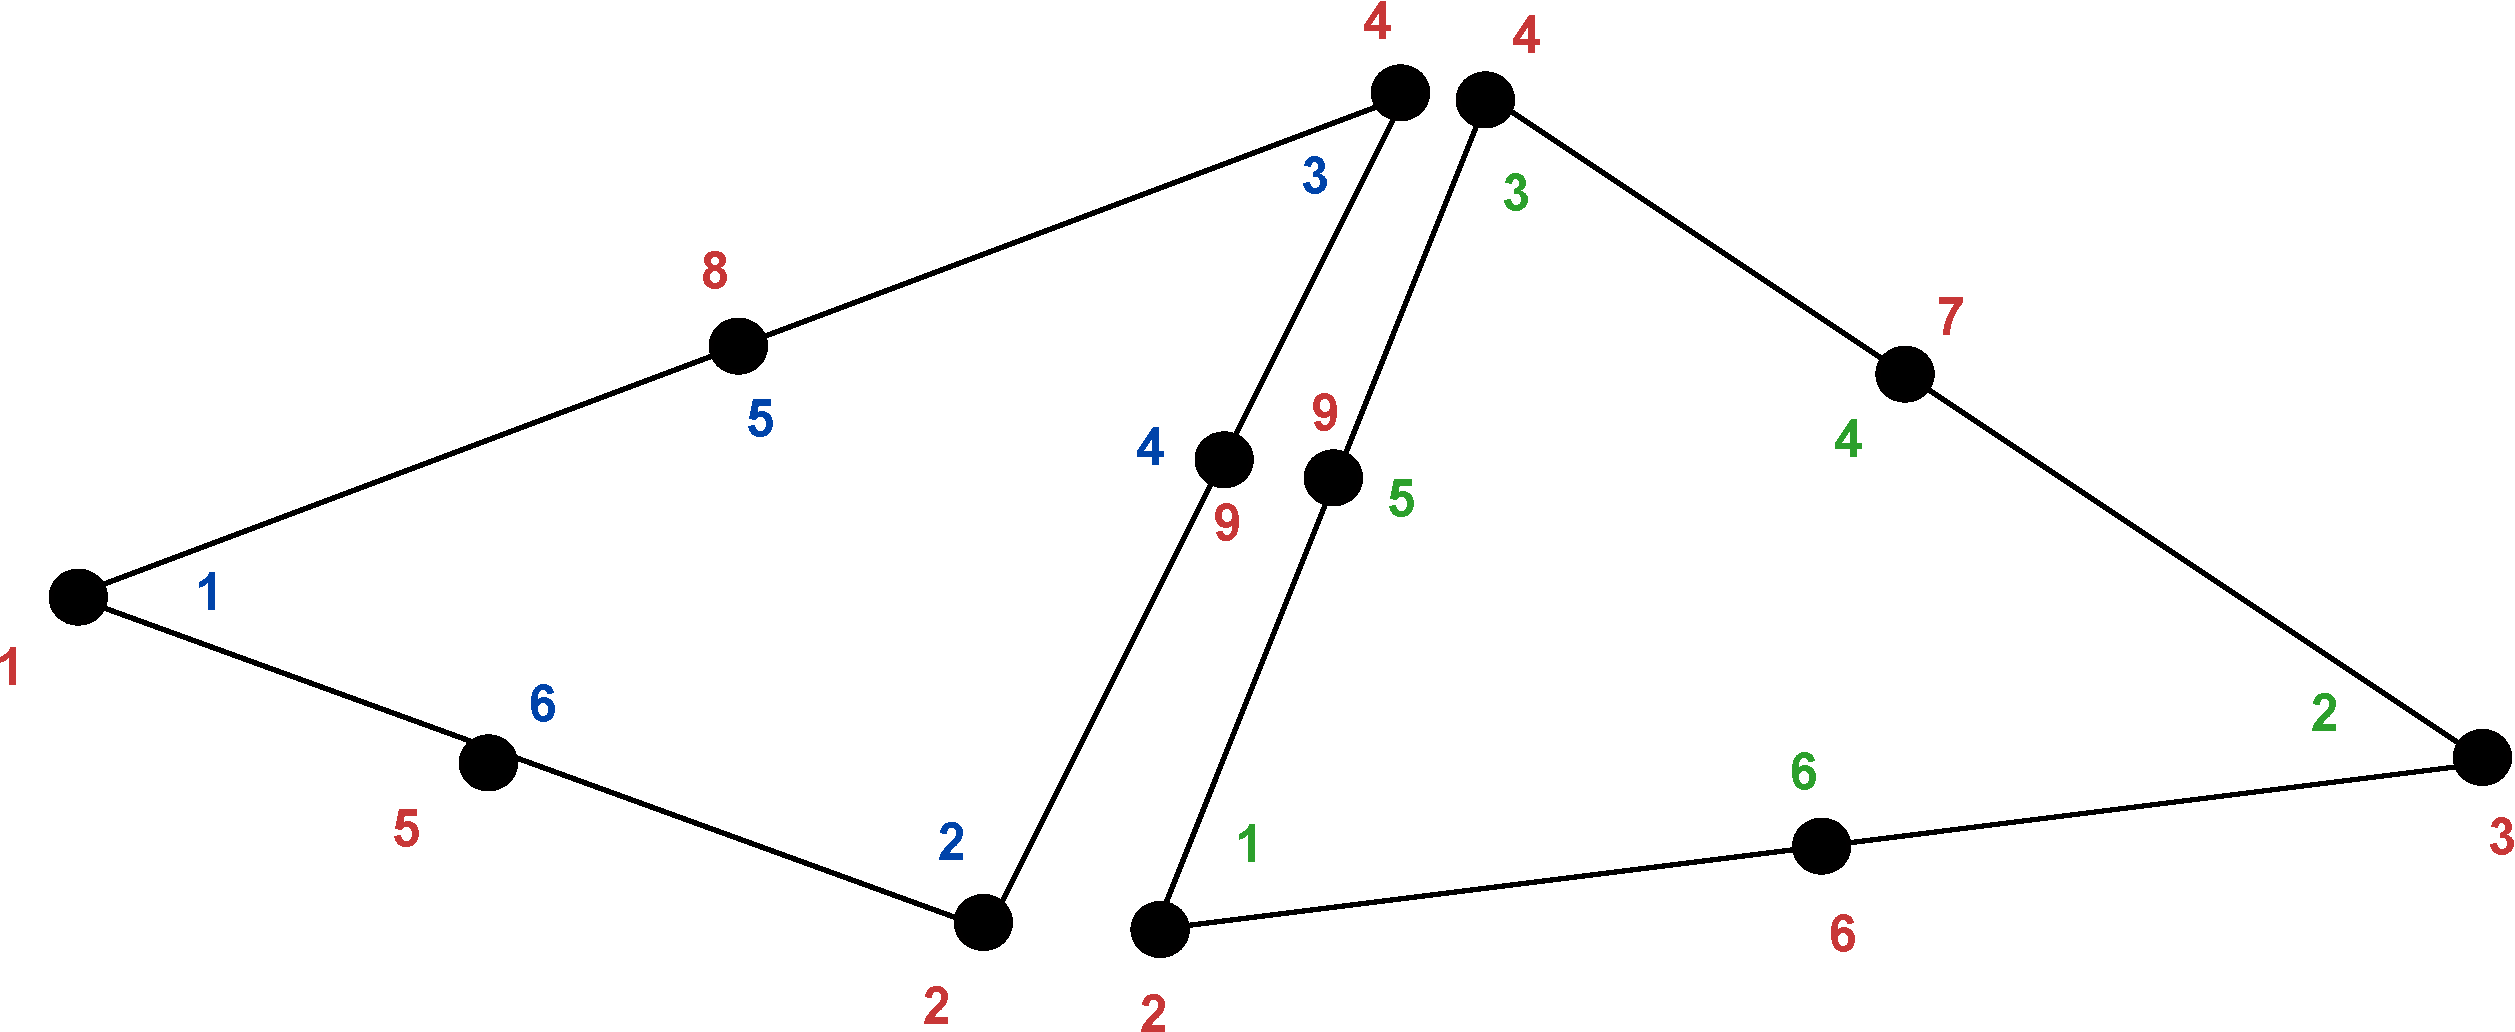
\includegraphics[width=10cm]{pdf/dofmap.pdf}
  \end{center}

\end{frame}

\begin{frame}
  \frametitle{The assembly algorithm}

  \begin{tabbing}
    $A = 0$ \\
    \\
    \textbf{for} $T \in \mathcal{T}$ \\
    \\
    \tab Compute the element matrix $A_T$ \\
    \\
    \tab Compute the local-to-global mapping $\iota_T$ \\
    \\
    \tab Add $A_T$ to $A$ according to $\iota_T$ \\
    \\
    \textbf{end for}
  \end{tabbing}

\end{frame}

\begin{frame}
  \frametitle{Adding the element matrix $A_T$}

  \begin{center}
    \def\svgwidth{\textwidth}
    \import{pdf/}{pdf/insertion.pdf_tex}
  \end{center}

\end{frame}


\fenicssection{Solving $AU = b$}

\begin{frame}
  \frametitle{Direct methods}

  \begin{itemize}
  \item
    Gaussian elimination
    \begin{itemize}
    \item
      Requires $\sim\frac{2}{3}N^3$ operations
    \end{itemize}
  \item
    LU factorization: $A = LU$
    \begin{itemize}
    \item
      Solve requires $\sim\frac{2}{3}N^3$ operations
    \item
      Reuse $L$ and $U$ for repeated solves
    \end{itemize}
  \item
    Cholesky factorization: $A = LL^{\top}$
    \begin{itemize}
    \item
      Works if $A$ is symmetric and positive definite
    \item
      Solve requires $\sim\frac{1}{3}N^3$ operations
    \item
      Reuse $L$ for repeated solves
    \end{itemize}
  \end{itemize}

\end{frame}

\begin{frame}
  \frametitle{Iterative methods}

  Krylov subspace methods
  \begin{itemize}
  \item
    GMRES (Generalized Minimal RESidual method)
  \item
    CG (Conjugate Gradient method)
    \begin{itemize}
    \item
      Works if $A$ is symmetric and positive definite
    \end{itemize}
  \item
    BiCGSTAB, MINRES, TFQMR, \ldots
  \end{itemize}

  Multigrid methods
  \begin{itemize}
  \item
    GMG (Geometric MultiGrid)
  \item
    AMG (Algebraic MultiGrid)
  \end{itemize}

  Preconditioners
  \begin{itemize}
  \item
    ILU, ICC, SOR, AMG, Jacobi, block-Jacobi, additive Schwarz, \ldots
  \end{itemize}

\end{frame}

\begin{frame}
  \frametitle{Which method should I use?}

  Rules of thumb
  \begin{itemize}
  \item
    Direct methods for small systems
  \item
    Iterative methods for large systems
  \item
    Break-even at ca 100--1000 degrees of freedom
  \item
    Use a symmetric method for a symmetric system
    \begin{itemize}
    \item
      Cholesky factorization (direct)
    \item
      CG (iterative)
    \end{itemize}
  \item
    Use a multigrid preconditioner for Poisson-like systems
  \item
    GMRES with ILU preconditioning is a good default choice
  \end{itemize}

\end{frame}

%\begin{frame}
  \frametitle{Current timings (2013--08--09)}

  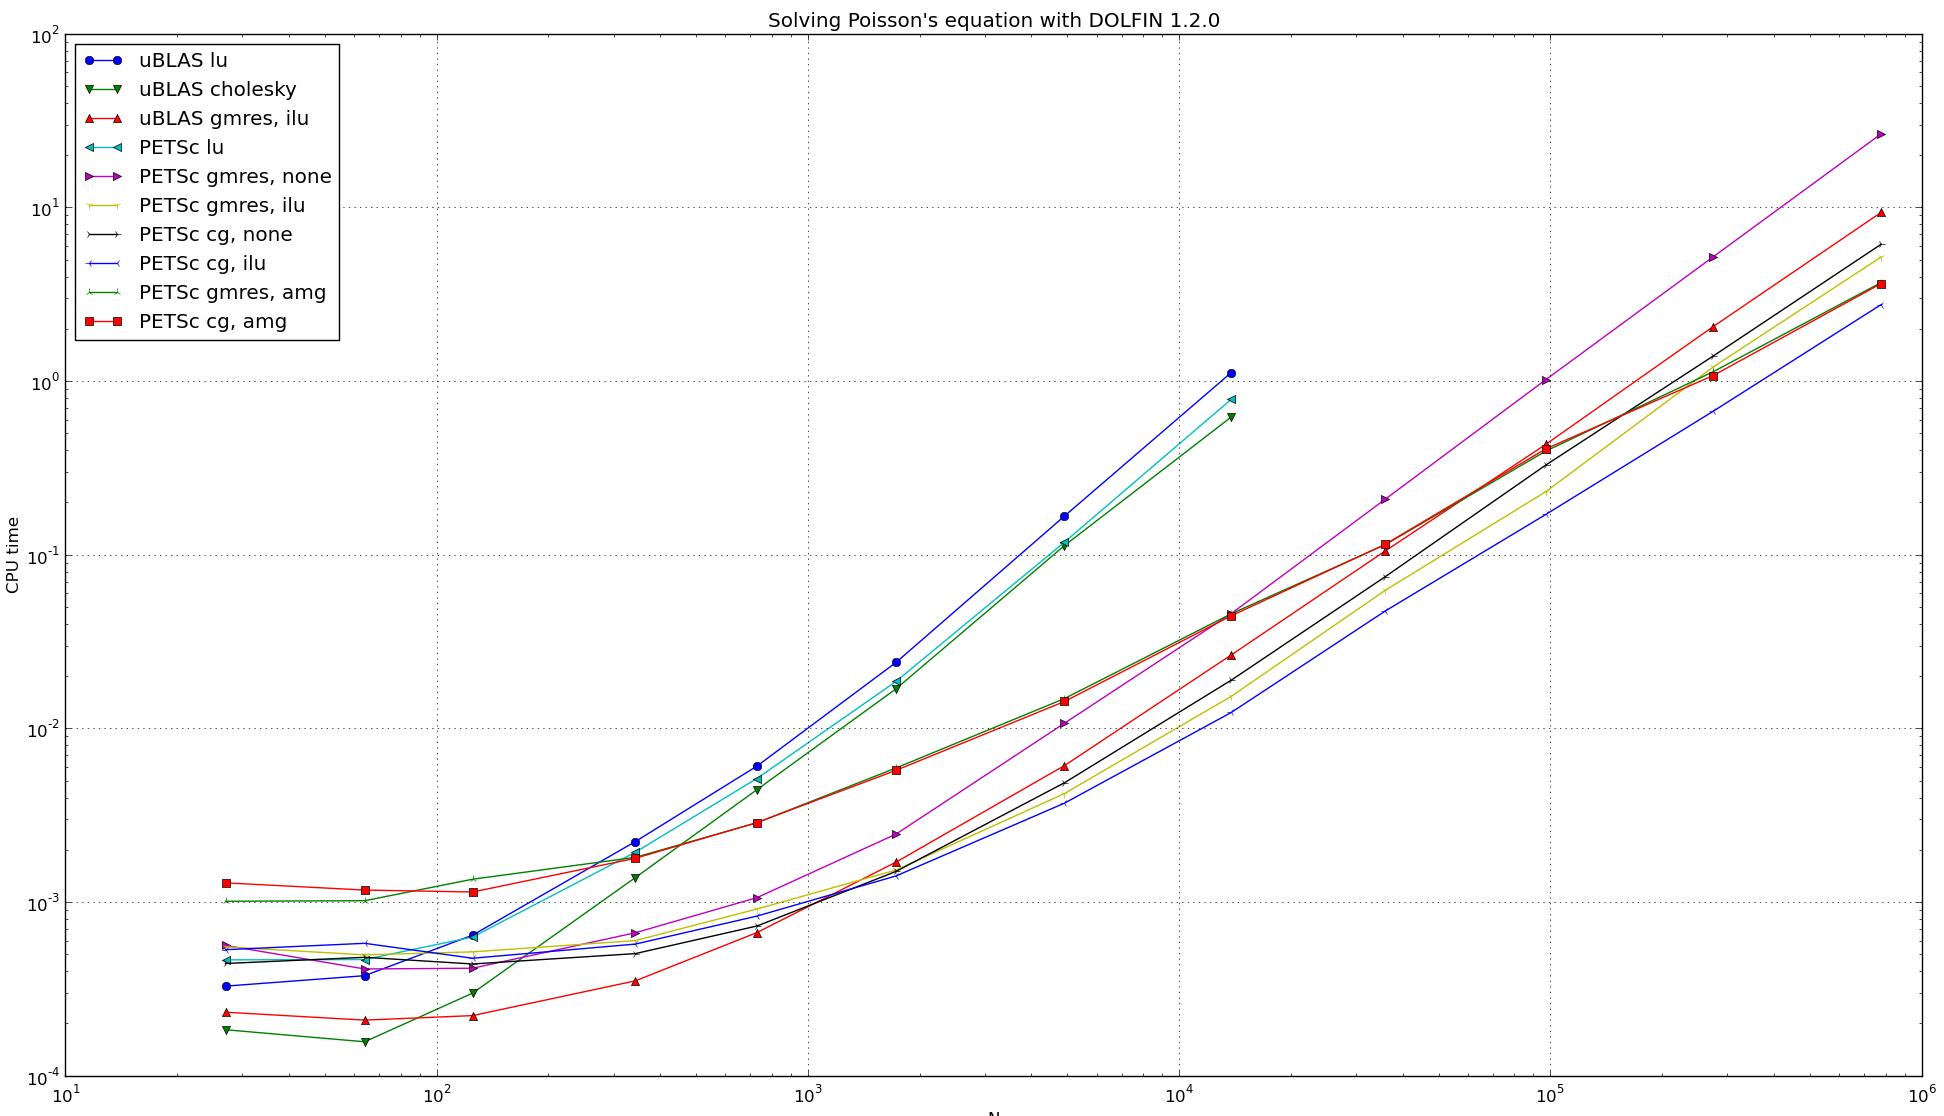
\includegraphics[width=\textwidth]{png/linear_algebra_timings.png}

\end{frame}


\begin{frame}
  \frametitle{A test problem}

  We construct a test problem for which we can easily check the
  answer. We first define the exact solution by
  \begin{equation*}
    u(x, y) = 1 + x^2 + 2y^2
  \end{equation*}

  \bigskip

  We insert this into Poisson's equation:

  \begin{equation*}
     f = -\Delta u = -\Delta (1 + x^2 + 2y^2) = -(2 + 4) = -6
  \end{equation*}

  \bigskip

  This technique is called the \emph{method of manufactured solutions}

\end{frame}

\begin{frame}[fragile]
  \frametitle{Implementation in FEniCS}
  \begin{python}
from fenics import *

mesh = UnitSquareMesh(8, 8)
V = FunctionSpace(mesh, "Lagrange", 1)

u0 = Expression("1 + x[0]*x[0] + 2*x[1]*x[1]", degree=2)
bc = DirichletBC(V, u0, "on_boundary")

f = Constant(-6.0)
u = TrialFunction(V)
v = TestFunction(V)
a = inner(grad(u), grad(v))*dx
L = f*v*dx

u = Function(V)
solve(a == L, u, bc)

plot(u)
interactive() # If using VTK plotting
  \end{python}

\end{frame}
 


\begin{frame}[fragile]
  \frametitle{Step by step: the first line}

  The first line of a FEniCS program usually begins with

  \begin{python}
from fenics import *
  \end{python}

  \bigskip

  This imports key classes like \emp{UnitSquareMesh}, \emp{FunctionSpace},
  \emp{Function} and so forth, from the FEniCS user interface
  (DOLFIN)

\end{frame}

\begin{frame}[fragile]
  \frametitle{Step by step: creating a mesh}

  Next, we create a mesh of our domain $\Omega$:
  \vspace{-1em}
  \begin{python}
mesh = UnitSquareMesh(8, 8)
  \end{python}
  This defines a mesh of $8 \times 8 \times 2 = 128$ triangles of the
  unit square.

  \bigskip

  Other useful classes for creating built-in meshes include
  \emp{UnitIntervalMesh},
  \emp{UnitCubeMesh},
  \emp{UnitCircleMesh},
  \emp{UnitSphereMesh},
  \emp{RectangleMesh} and
  \emp{BoxMesh}

  \bigskip

  More complex geometries can be built using Constructive Solid
  Geometry (CSG) through the FEniCS component \emp{mshr}:
  \vspace{-1em}
  \begin{python}
from mshr import *
r = Rectangle(Point(0.5, 0.5), Point(1.5, 1.5))
c = Circle(Point(1.0, 1.0), 0.2)
g = r - c
mesh = generate_mesh(g, 10)
  \end{python}

  \normalsize

\end{frame}

\begin{frame}[fragile]
  \frametitle{Step by step: creating a function space}

  The following line creates a finite element function space relative to this mesh:
\vspace{-1em}
\begin{python}
V = FunctionSpace(mesh, "Lagrange", 1)
\end{python}

  \bigskip

  The second argument specifies the type of element, while the third
  argument is the degree of the basis functions on the element

  \bigskip

  Other types of elements include
  \emp{"Discontinuous Lagrange"},
  \emp{"Brezzi-Douglas-Marini"},
  \emp{"Raviart-Thomas"},
  \emp{"Crouzeix-Raviart"},
  \emp{"Nedelec 1st kind H(curl)"} and
  \emp{"Nedelec 2nd kind H(curl)"}

\end{frame}

\begin{frame}[fragile]
  \frametitle{Step by step: defining expressions}

  Next, we define an expression for the boundary value:
  \vspace{-1em}
  \begin{python}
u0 = Expression("1 + x[0]*x[0] + 2*x[1]*x[1]", degree=2)
  \end{python}
  The formula must be written in C++ syntax, and
  the polynomial degree must be specified.

  \bigskip

  The \emp{Expression} class is very flexible and can be used to
  create complex user-defined expressions. For more information, try
\vspace{-1em}
  \begin{python}
from fenics import *
help(Expression)
  \end{python}
  in Python or, in the shell:
  \vspace{-1em}
  \begin{python}
$ pydoc fenics.Expression
  \end{python}

\end{frame}


\begin{frame}[fragile]
  \frametitle{Step by step: defining a boundary condition}

  The following code defines a Dirichlet boundary condition:
\vspace{-1em}
\begin{python}
bc = DirichletBC(V, u0, "on_boundary")
\end{python}

  This boundary condition states that a function in the function space
  defined by \emp{V} should be equal to \emp{u0} on the domain defined
  by \emp{"on\_boundary"}

  \bigskip

  Note that the above line does not yet apply the boundary condition
  to all functions in the function space

\end{frame}

\begin{frame}[fragile, shrink=5]
  \frametitle{Step by step: more about defining domains}
  For a Dirichlet boundary condition, a simple domain can be defined
  by a string
  \vspace{-1em}
  \begin{python}
"on_boundary" # The entire boundary
  \end{python}

  Alternatively, domains can be defined by subclassing \emp{SubDomain}
  \vspace{-1em}
  \begin{python}
class Boundary(SubDomain):
    def inside(self, x, on_boundary):
        return on_boundary
  \end{python}

  You may want to experiment with the definition of the boundary:
  \vspace{-1em}
  \begin{python}
"near(x[0], 0.0)" # x_0 = 0
"near(x[0], 0.0) || near(x[1], 1.0)"
  \end{python}

  There are many more possibilities, see
  \vspace{-1em}
  \begin{python}
help(SubDomain)
help(DirichletBC)
  \end{python}

\end{frame}
    

\begin{frame}[fragile]
  \frametitle{Step by step: defining the right-hand side}

  The right-hand side $f = - 6$ may be defined as follows:
  \begin{python}
f = Expression("-6.0", degree=0)
  \end{python}

  \bigskip

  or (more efficiently) as
  \begin{python}
f = Constant(-6.0)
  \end{python}

\end{frame}

\begin{frame}[fragile]
  \frametitle{Step by step: defining variational problems}

  Variational problems are defined in terms of \emph{trial} and
  \emph{test} functions:
  \begin{python}
u = TrialFunction(V)
v = TestFunction(V)
  \end{python}

  \bigskip

  We now have all the objects we need in order to specify the bilinear
  form $a(u,v)$ and the linear form $L(v)$:
  \begin{python}
a = inner(grad(u), grad(v))*dx
L = f*v*dx
  \end{python}

\end{frame}

\begin{frame}[fragile]
  \frametitle{Step by step: solving variational problems}

  Once a variational problem has been defined, it may be solved
  by calling the \emp{solve} function:

  \begin{python}
u = Function(V)
solve(a == L, u, bc)
  \end{python}

  \bigskip

  Note the reuse of the variable name \emp{u} as both a \emp{TrialFunction}
  in the variational problem and a \emp{Function} to store the solution.

\end{frame}

% \begin{frame}[fragile]
  \frametitle{Step by step: post-processing}

  The solution and the mesh may be plotted by simply calling:
  \vspace{-0.25cm}
  \begin{python}
plot(u)
plot(mesh)
interactive()
  \end{python}

  \bigskip

  The \emp{interactive()} call is necessary for the plot to remain on the
  screen and allows the plots to be rotated, translated and zoomed

  \bigskip

  For postprocessing in ParaView or MayaVi, store the solution in VTK
  format:
  \begin{python}
file = File("poisson.pvd")
file << u
  \end{python}

\end{frame}
 Uncomment this if you use VTK plotting
\begin{frame}[fragile]
  \frametitle{Step by step: post-processing using Notebooks}

  Add these incantations on top (after importing dolfin/fenics)
  \vspace{-1em}
  \begin{python}
import pylab
%matplotlib inline
parameters["plotting_backend"] = "matplotlib"
    \end{python}

  The solution and the mesh may be plotted by simply calling:
  \vspace{-1em}
  \begin{python}
plot(u)
pylab.show()
plot(mesh)
pylab.show()
  \end{python}

  For postprocessing in ParaView or MayaVi, store the solution in VTK
  format:
  \vspace{-1em}
  \begin{python}
file = File("poisson.pvd")
file << u
  \end{python}

\end{frame}


% Comment this next slide out if you are confident that the students
% know how to write and run a Python program, or if you are using
% e.g. Notebooks
% \begin{frame}[fragile]
\frametitle{Python/FEniCS programming 101}

\begin{enumerate}
\item
  Open a file with your favorite text editor (Emacs :-) ) and name the
  file something like \texttt{test.py}
  \bigskip
\item
  Write the following in the file and save it:
\vspace{-1em}
  \begin{python}
from fenics import *
print(dolfin.__version__)
  \end{python}
  \bigskip
\item
  Run the file/program by typing the following in a terminal (with
  FEniCS setup):
\vspace{-1em}
 \begin{python}
$ python test.py
 \end{python}
\end{enumerate}

\end{frame}







\end{document}
